% Use only LaTeX2e, calling the article.cls class and 12-point type.

\documentclass[12pt]{article}

\usepackage{polski}
\usepackage[utf8]{inputenc}


% Users of the {thebibliography} environment or BibTeX should use the
% scicite.sty package, downloadable from *Science* at
% www.sciencemag.org/about/authors/prep/TeX_help/ .
% This package should properly format in-text
% reference calls and reference-list numbers.

\usepackage{scicite}

% Use times if you have the font installed; otherwise, comment out the
% following line.

\usepackage{times}

% The preamble here sets up a lot of new/revised commands and
% environments.  It's annoying, but please do *not* try to strip these
% out into a separate .sty file (which could lead to the loss of some
% information when we convert the file to other formats).  Instead, keep
% them in the preamble of your main LaTeX source file.


% The following parameters seem to provide a reasonable page setup.

\topmargin 0.0cm
\oddsidemargin 0.2cm
\textwidth 16cm 
\textheight 21cm
\footskip 1.0cm


%The next command sets up an environment for the abstract to your paper.

\newenvironment{sciabstract}{%
\begin{quote} \bf}
{\end{quote}}


% If your reference list includes text notes as well as references,
% include the following line; otherwise, comment it out.

\renewcommand\refname{References and Notes}

% The following lines set up an environment for the last note in the
% reference list, which commonly includes acknowledgments of funding,
% help, etc.  It's intended for users of BibTeX or the {thebibliography}
% environment.  Users who are hand-coding their references at the end
% using a list environment such as {enumerate} can simply add another
% item at the end, and it will be numbered automatically.

\newcounter{lastnote}
\newenvironment{scilastnote}{%
\setcounter{lastnote}{\value{enumiv}}%
\addtocounter{lastnote}{+1}%
\begin{list}%
{\arabic{lastnote}.}
{\setlength{\leftmargin}{.22in}}
{\setlength{\labelsep}{.5em}}}
{\end{list}}


% Include your paper's title here

\title{Użycie hybrydowego Algorytmu Genetycznego z Symulowanym Wyżarzaniem w celu znajdowania minimalnych drzew rozpinających w wariancie kwadratowym} 


% Place the author information here.  Please hand-code the contact
% information and notecalls; do *not* use \footnote commands.  Let the
% author contact information appear immediately below the author names
% as shown.  We would also prefer that you don't change the type-size
% settings shown here.

\author
{Michał Drzał\\Marcin Paśko\\
\\
\normalsize{Akademia Górniczo-Hutnicza im. Adama Mickiewicza w Krakowie}\\
\normalsize{Wydział Informatyki Elektroniki i Telekomunikacji}\\
}

% Include the date command, but leave its argument blank.

\date{}



%%%%%%%%%%%%%%%%% END OF PREAMBLE %%%%%%%%%%%%%%%%



\begin{document} 

% Double-space the manuscript.

\baselineskip24pt

% Make the title.

\maketitle 



% Place your abstract within the special {sciabstract} environment.

\begin{sciabstract}
  Niniejszy dokument stanowi raport z wynikami projektu, relalizowanego z przedmiotu Stochastyczne Algorytmy Obliczeniowe, prowadzonego przed prof. dr hab. inż. Roberta Shaefera.
\end{sciabstract}



% In setting up this template for *Science* papers, we've used both
% the \section* command and the \paragraph* command for topical
% divisions.  Which you use will of course depend on the type of paper
% you're writing.  Review Articles tend to have displayed headings, for
% which \section* is more appropriate; Research Articles, when they have
% formal topical divisions at all, tend to signal them with bold text
% that runs into the paragraph, for which \paragraph* is the right
% choice.  Either way, use the asterisk (*) modifier, as shown, to
% suppress numbering.

\section*{Wstęp}





\section{Sformułowanie problemu}

Niech $G =(V,E)$ bedzie nieskierowanym grafem ze zbiorem wierzcholkow V i zbiorem krawedzi E. Problem kwadratowego minimalnego drzewa rozpinajacego (QMSTP, quadratic minimum spanning tree). Kazda krawedz posiada przypisany koszt $e_{g}$ oraz każda para krawedzi posiada koszt $c_{eg}$. Minimalizowany koszt drzewa rozpinajacego $T= (V, E(T))$ jest wyrazony:
$$ F(T) = \sum_{e \in E(T) } c_e + \sum_{(e,g) \in \Psi (T)} c_{eg} $$

 $\Psi (T)$ oznacza zbior wszystkich par krawedzi znajdujacych sie w drzewie $T$. Rozwiazania QMSTP znajduja zastosowanie w telekomunikacji, logistyce i dystrybucji energii.
 
 Problem QMST jest NP-trudny \cite{Assad}, przez co optymalny algorytm rozwiazujacy go w czasie wielomianowym istnieje tylko jesli $P=NP$. Uzasadnione jest wiec wykorzystanie do znalezienia rozwiazania jednej z wielu dostepnych metaheurystyk.
 
 \section{Wykorzystana metaheurystyka}

Zastosowanie regul zaczerpnietych z procesow ewolucyjnych jest powszechnie stosowana praktyka podczas rozwiazywania problemow ewolucyjnych. Na potrzeby naszego projektu wykorzystalismy algorytm genetyczny jako matryce do stworzenia wlasciwego algorytmu. W trakcie rozwiazywania QMSTP utrzymujemy populacje rozwiazan, gdzie pojedynczy osobnik stanowi pojedyncze drzewo rozpinajace w grafie $G$. Reprezentowany jest w postaci grafu odpowiadajacego liscie krawedzi z oryginalnego grafu. Korzystajac z wzoru na koszt drzewa rozpinajacego ustalana jest jakosc rozwiazania. Nastepnie droga selekcji turniejowej wybierane sa rozwiazania do krzyzowania. Rozwiazania powstale wskutek krzyzowania zamieniaja najslabsze rozwiazania z populacji. Oprocz krzyzowania rozwiazania z pewnym prawdopodbienstwem poddawane sa operacji losowej mutacji.


W celu ustalenia poczatkowej populacji konieczne jest wygenerowanie losowych grafow bedacych drzewami rozpinajacymi (niekoniecznie losowymi). Wazne jest aby rozklad z ktorego losowane sa drzewa rozpinajace byl rozkladem jednostajnym, dzieki czemu mozliwe bedzie przeszukiwanie przestrzeni rozwiazan bez uprzywilejowanego traktowania czesci rozwiazan. Losowe drzewo rozpinajace uzyskuje sie rozpoczynajac bladzenie losowe zaczynajac od losowego wierzcholka. 

\begin{figure}[h!]
 \centering
\begin{algorithmic}
\Function{RandomTree}{} 
\State $r\gets \Call{RandomVertex}{nil}$
\For{ $i < n$} 
	\State $InTree[i] \gets false $
	\State $i\gets i+1$
\EndFor
\State $Next[r] \gets nil $
\State $InTree[r] \gets true $


\For{ $i < n$} 
	\State $u \gets 1 $
    \While{not InTree[u]} 
    	\State $Next[u] \gets \Call{RandomSuccessor}{u}$
        \State $u \gets Next[u]$
    \EndWhile
    \State $u\gets i$
    \While{not InTree[u]} 
    	\State $InTree[u] \gets true$
        \State $u \gets Next[u]$
    \EndWhile
    
	\State $i\gets i+1$
\EndFor


\Return Next

\EndFunction

\end{algorithmic}
\caption{Algorytm generujacy losowe drzewo rozpinajace}
\end{figure}





W projekcie wykorzystano rowniez mechanizmy zaczerpniete z algorytmu symulowanego wyzarzania. Jest to algorytm wzorowany procesie wyzarzania stosowanego w metalurgii. Opiera sie ono o stopniowym, kontrolowanym zmniejszaniu temperatury metalu celem optymalizacji (minimalizacji) energii swobodnej materialu. Opierajac sie na tym mechanizmie, czesc parametrow procesu ewolucyjnego rowniez podlega procesowi powolnej zmiany wedlug ustalonego planu, naleza do nich:

\begin{itemize}
  \item prawdopodobienstwo mutacji
  \item wielkosc turnieju
  \item The third etc \ldots
\end{itemize}




 \section{Zbior testowy i wyniki}


 Do testow wykorzystano benchmark udstepniony przez Roberto Cordone. Zawiera on zbior grafow rozniacych sie od siebie:
 
 \begin{itemize}
  \item iloscia wierzcholkow (od 10 do 50 wierzchołków)
  \item gestoscia grafow ($\frac{1}{3}, \frac{2}{3}, 1$)
  \item zakresem kosztow krawedzi i kosztow pomiedzy parami krawedzi (dwa dyskretne zakresy: 1-10,1-100) 
\end{itemize}

Do testow zostaly wybrane 3 grafy odpowiednio z: 10, 15 i 20 wierzcholkami. Wszystkie grafy sa grafami pelnymi oraz wartosci kosztow znajduja sie w wiekszym zakresie: 1-100. Dysponujemy dla nich rowniez najlepszymi uzyskanymi rezultatami, odpowiednio: 2197, 5879 i 11101.


\begin{thebibliography}{9}

\bibitem{Assad}
  A. Assad, W. Xu,
  \emph{The quadratic minimum spanning tree problem.}.
  Naval Research Logistics, 1992,Vol.39, 399–417.

\end{thebibliography}


\section*{Wyniki}

Niniejszy rozdział stanowi prezentację wyników. Wykonaliśmy łącznie 3 eksperymenty, każdy dla 3 rozmiarów danych. Wyniki w każdym przypadku zostały uśrednione dla 3 przebiegów. Na każdym wykresie przedstawiono wagę drzewa dla przeciętnego osobnika w populacji. Os X stanowi ilość ewaluacji funkcji celu.

Poniższe trzy wykresy stanowią przypadek porównawczy dla zwykłego algorytmu genetycznego z selekcją turniejową.

Mały rozmiar danych:

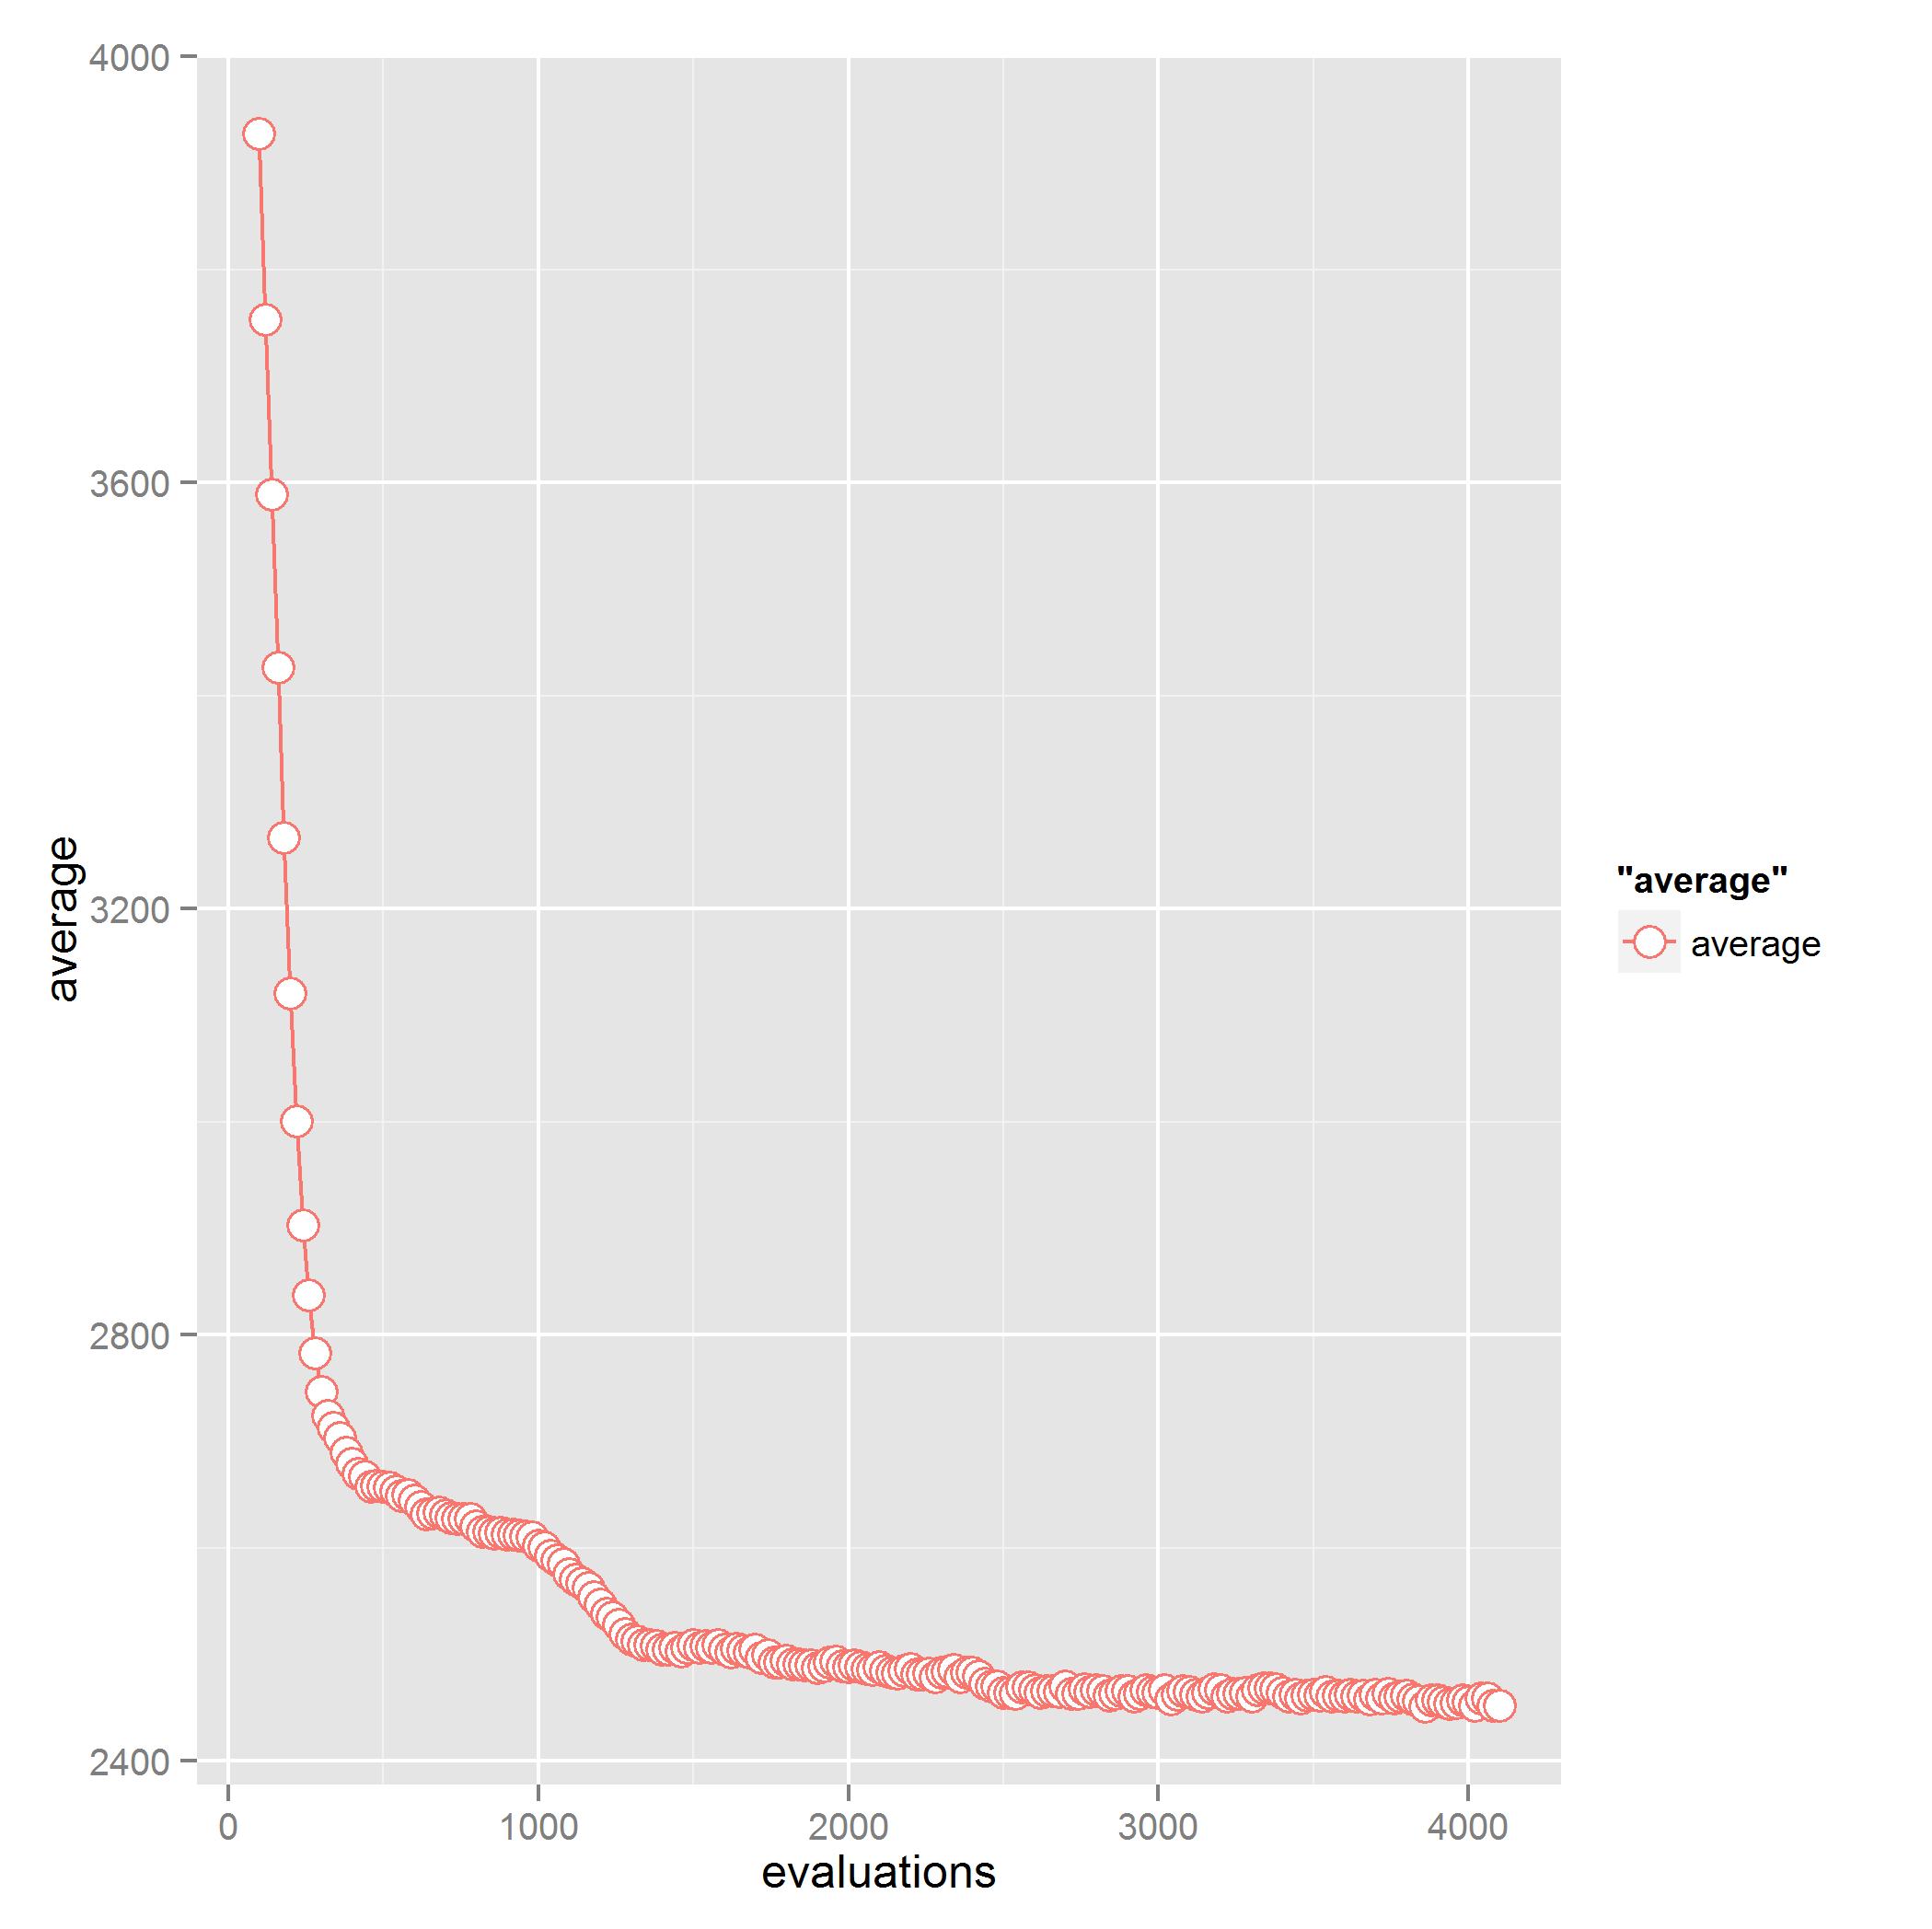
\includegraphics[]{simple_graph0.png}

Średni rozmiar danych:

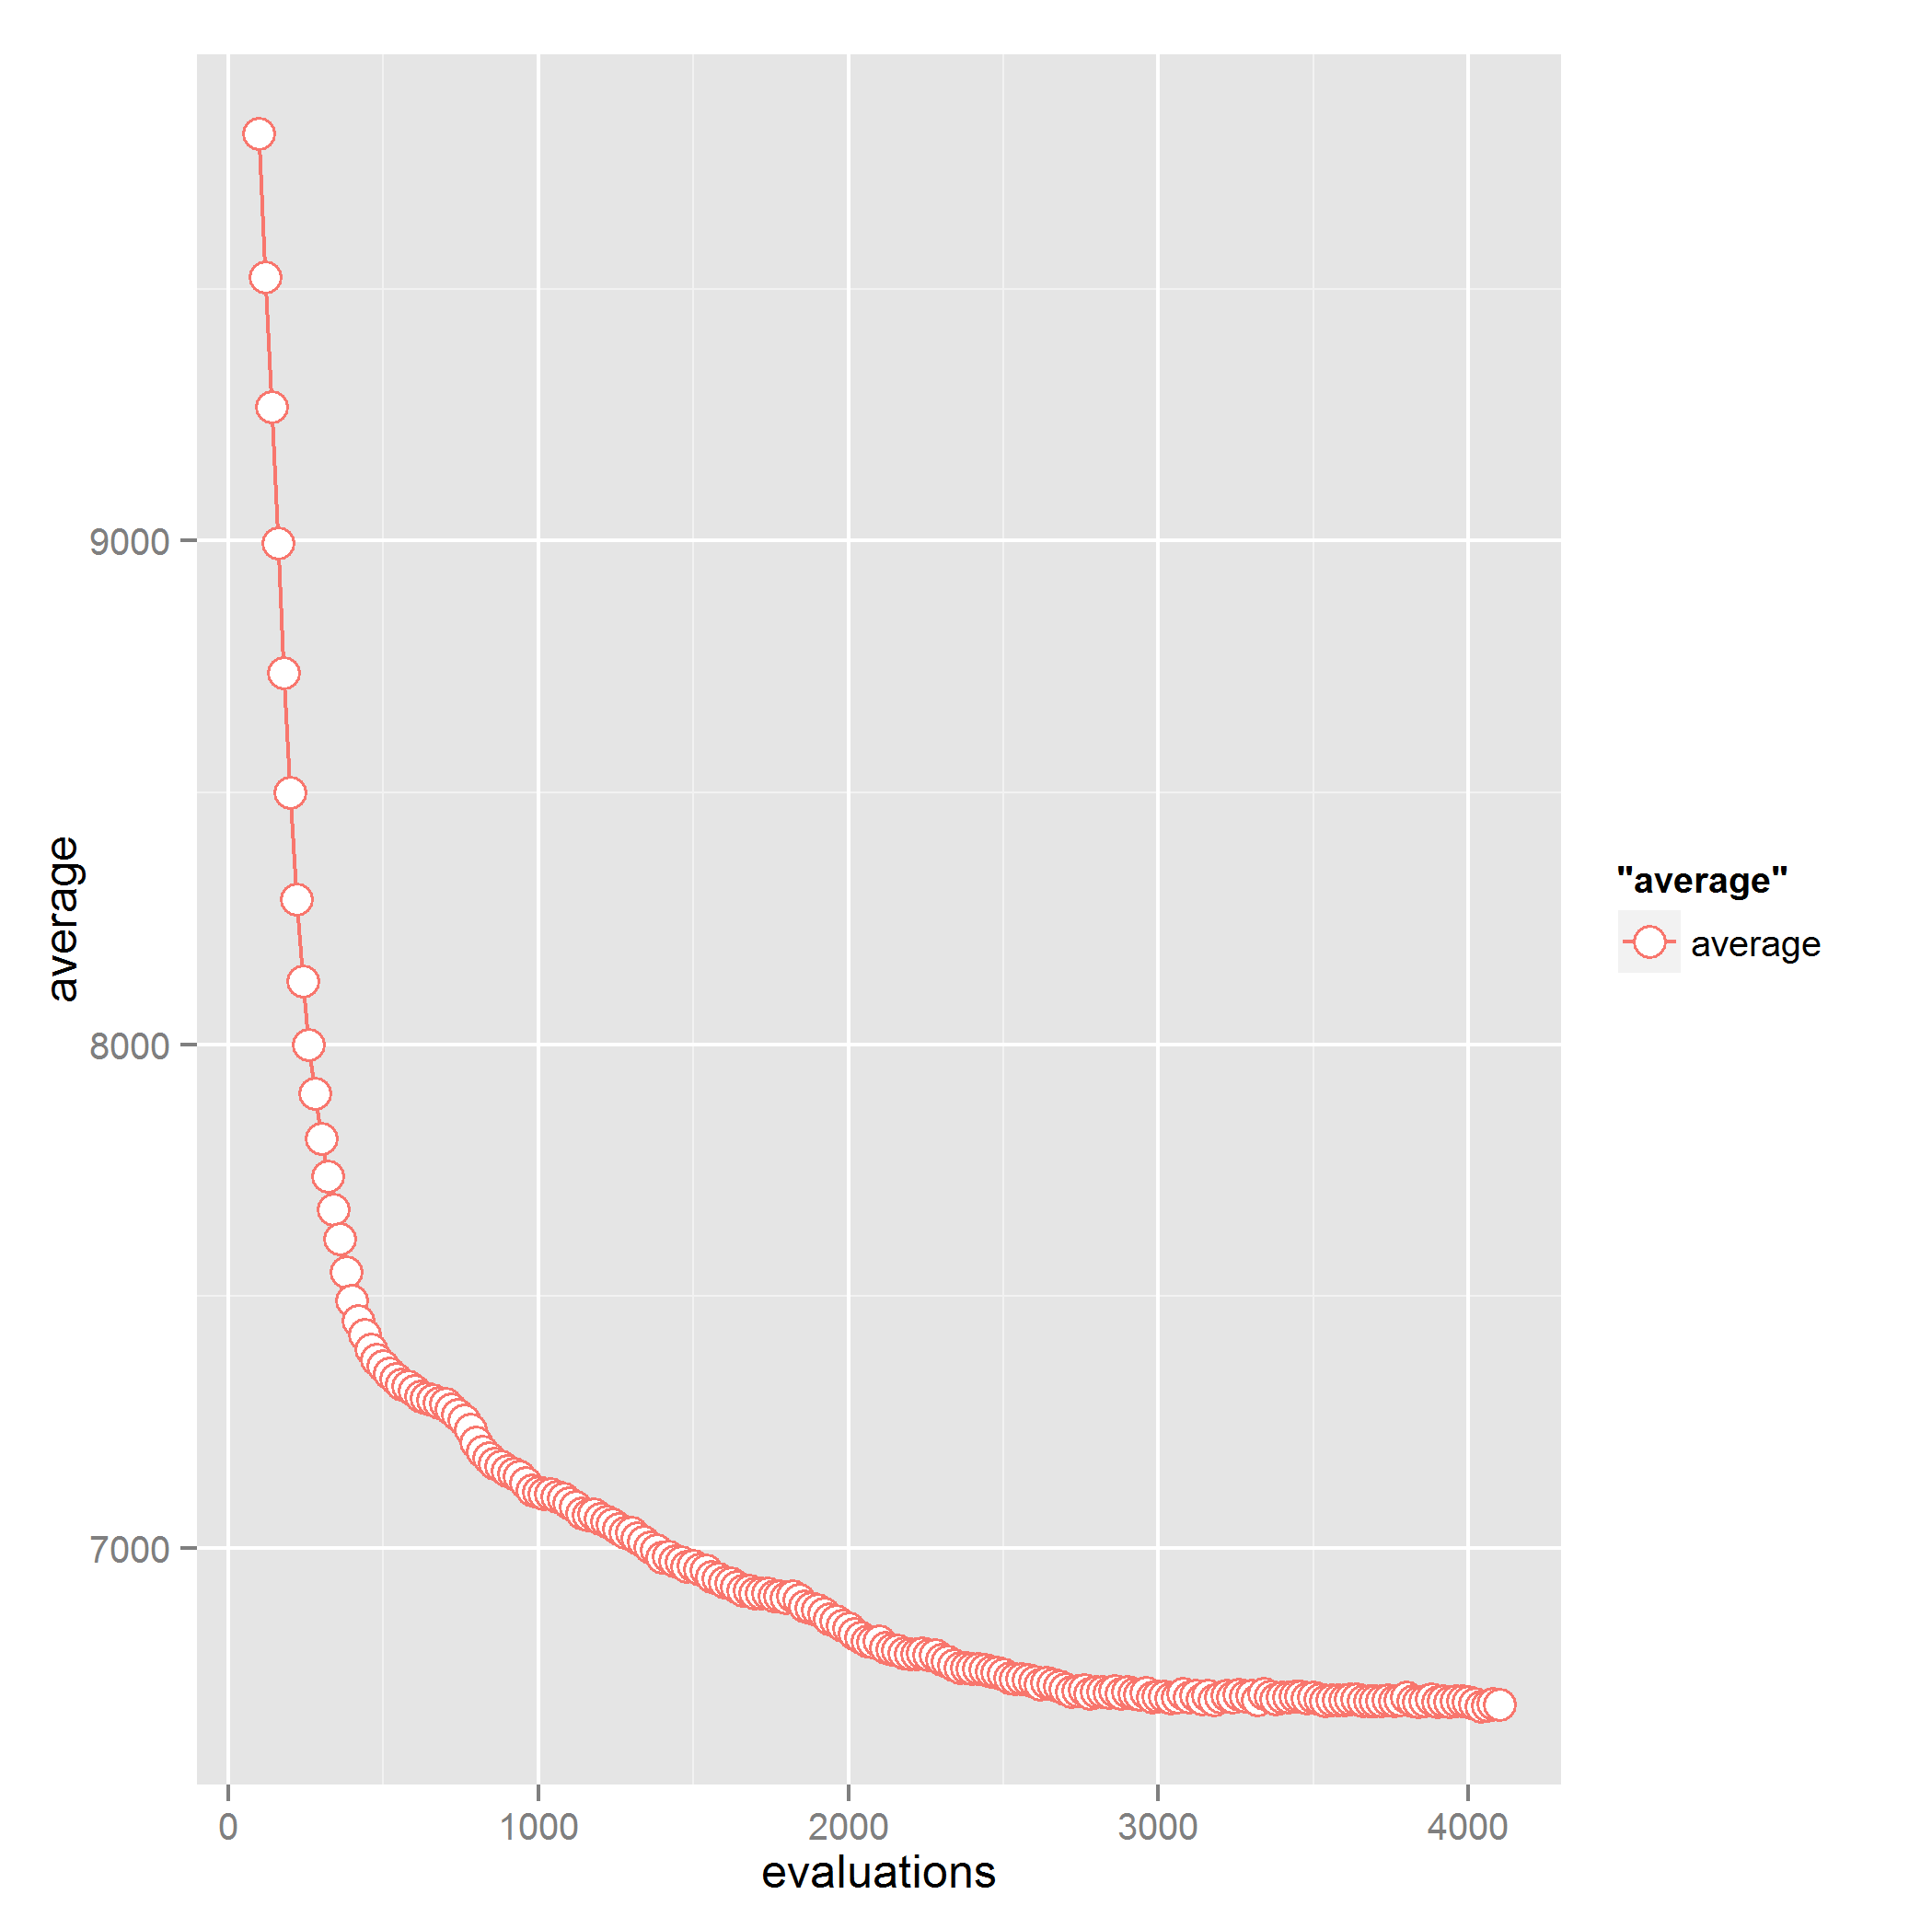
\includegraphics[]{simple_graph1.png}

Duży rozmiar danych:

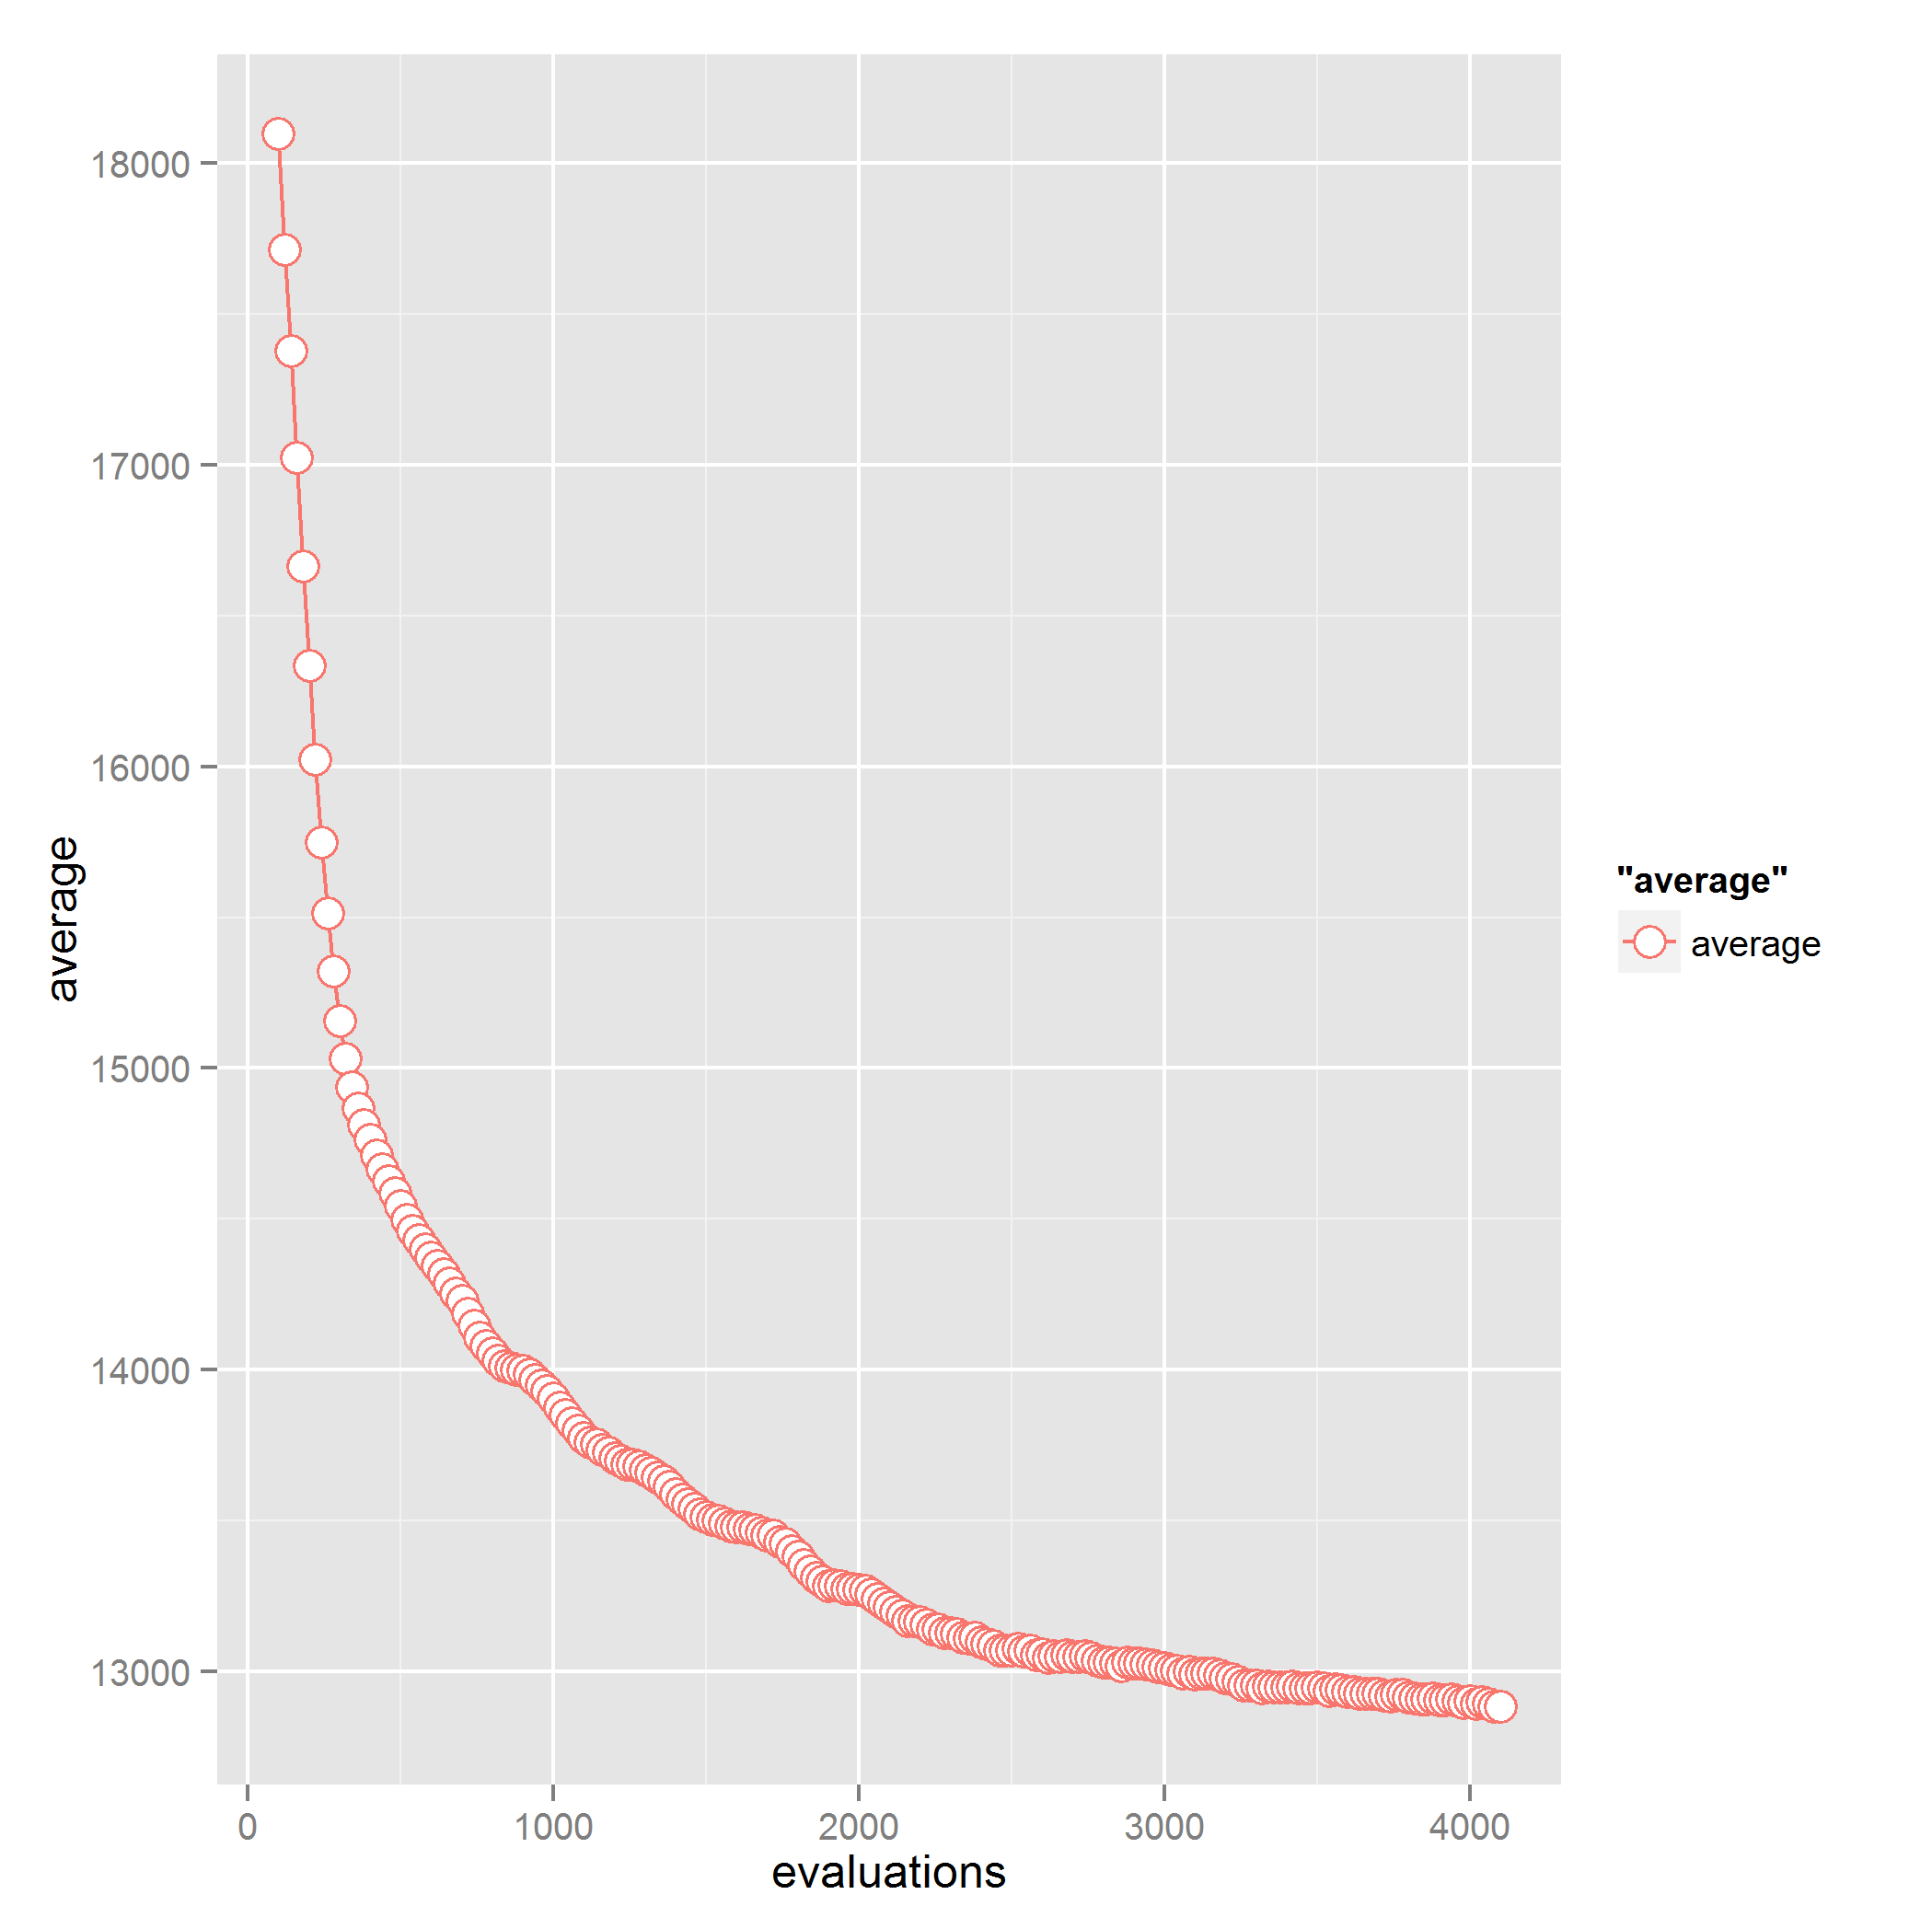
\includegraphics[]{simple_graph2.png}

Kolejne wyniki pochodzą z hybrydy algorytmu symulowanego wyżarzania, gdzie wychładzamy prawdopodobieństwo mutacji, które na początku miało dużą wartość np 1, a następnie jest wychładzane wykładniczo do bardzo małej wartości.

Mały rozmiar danych:

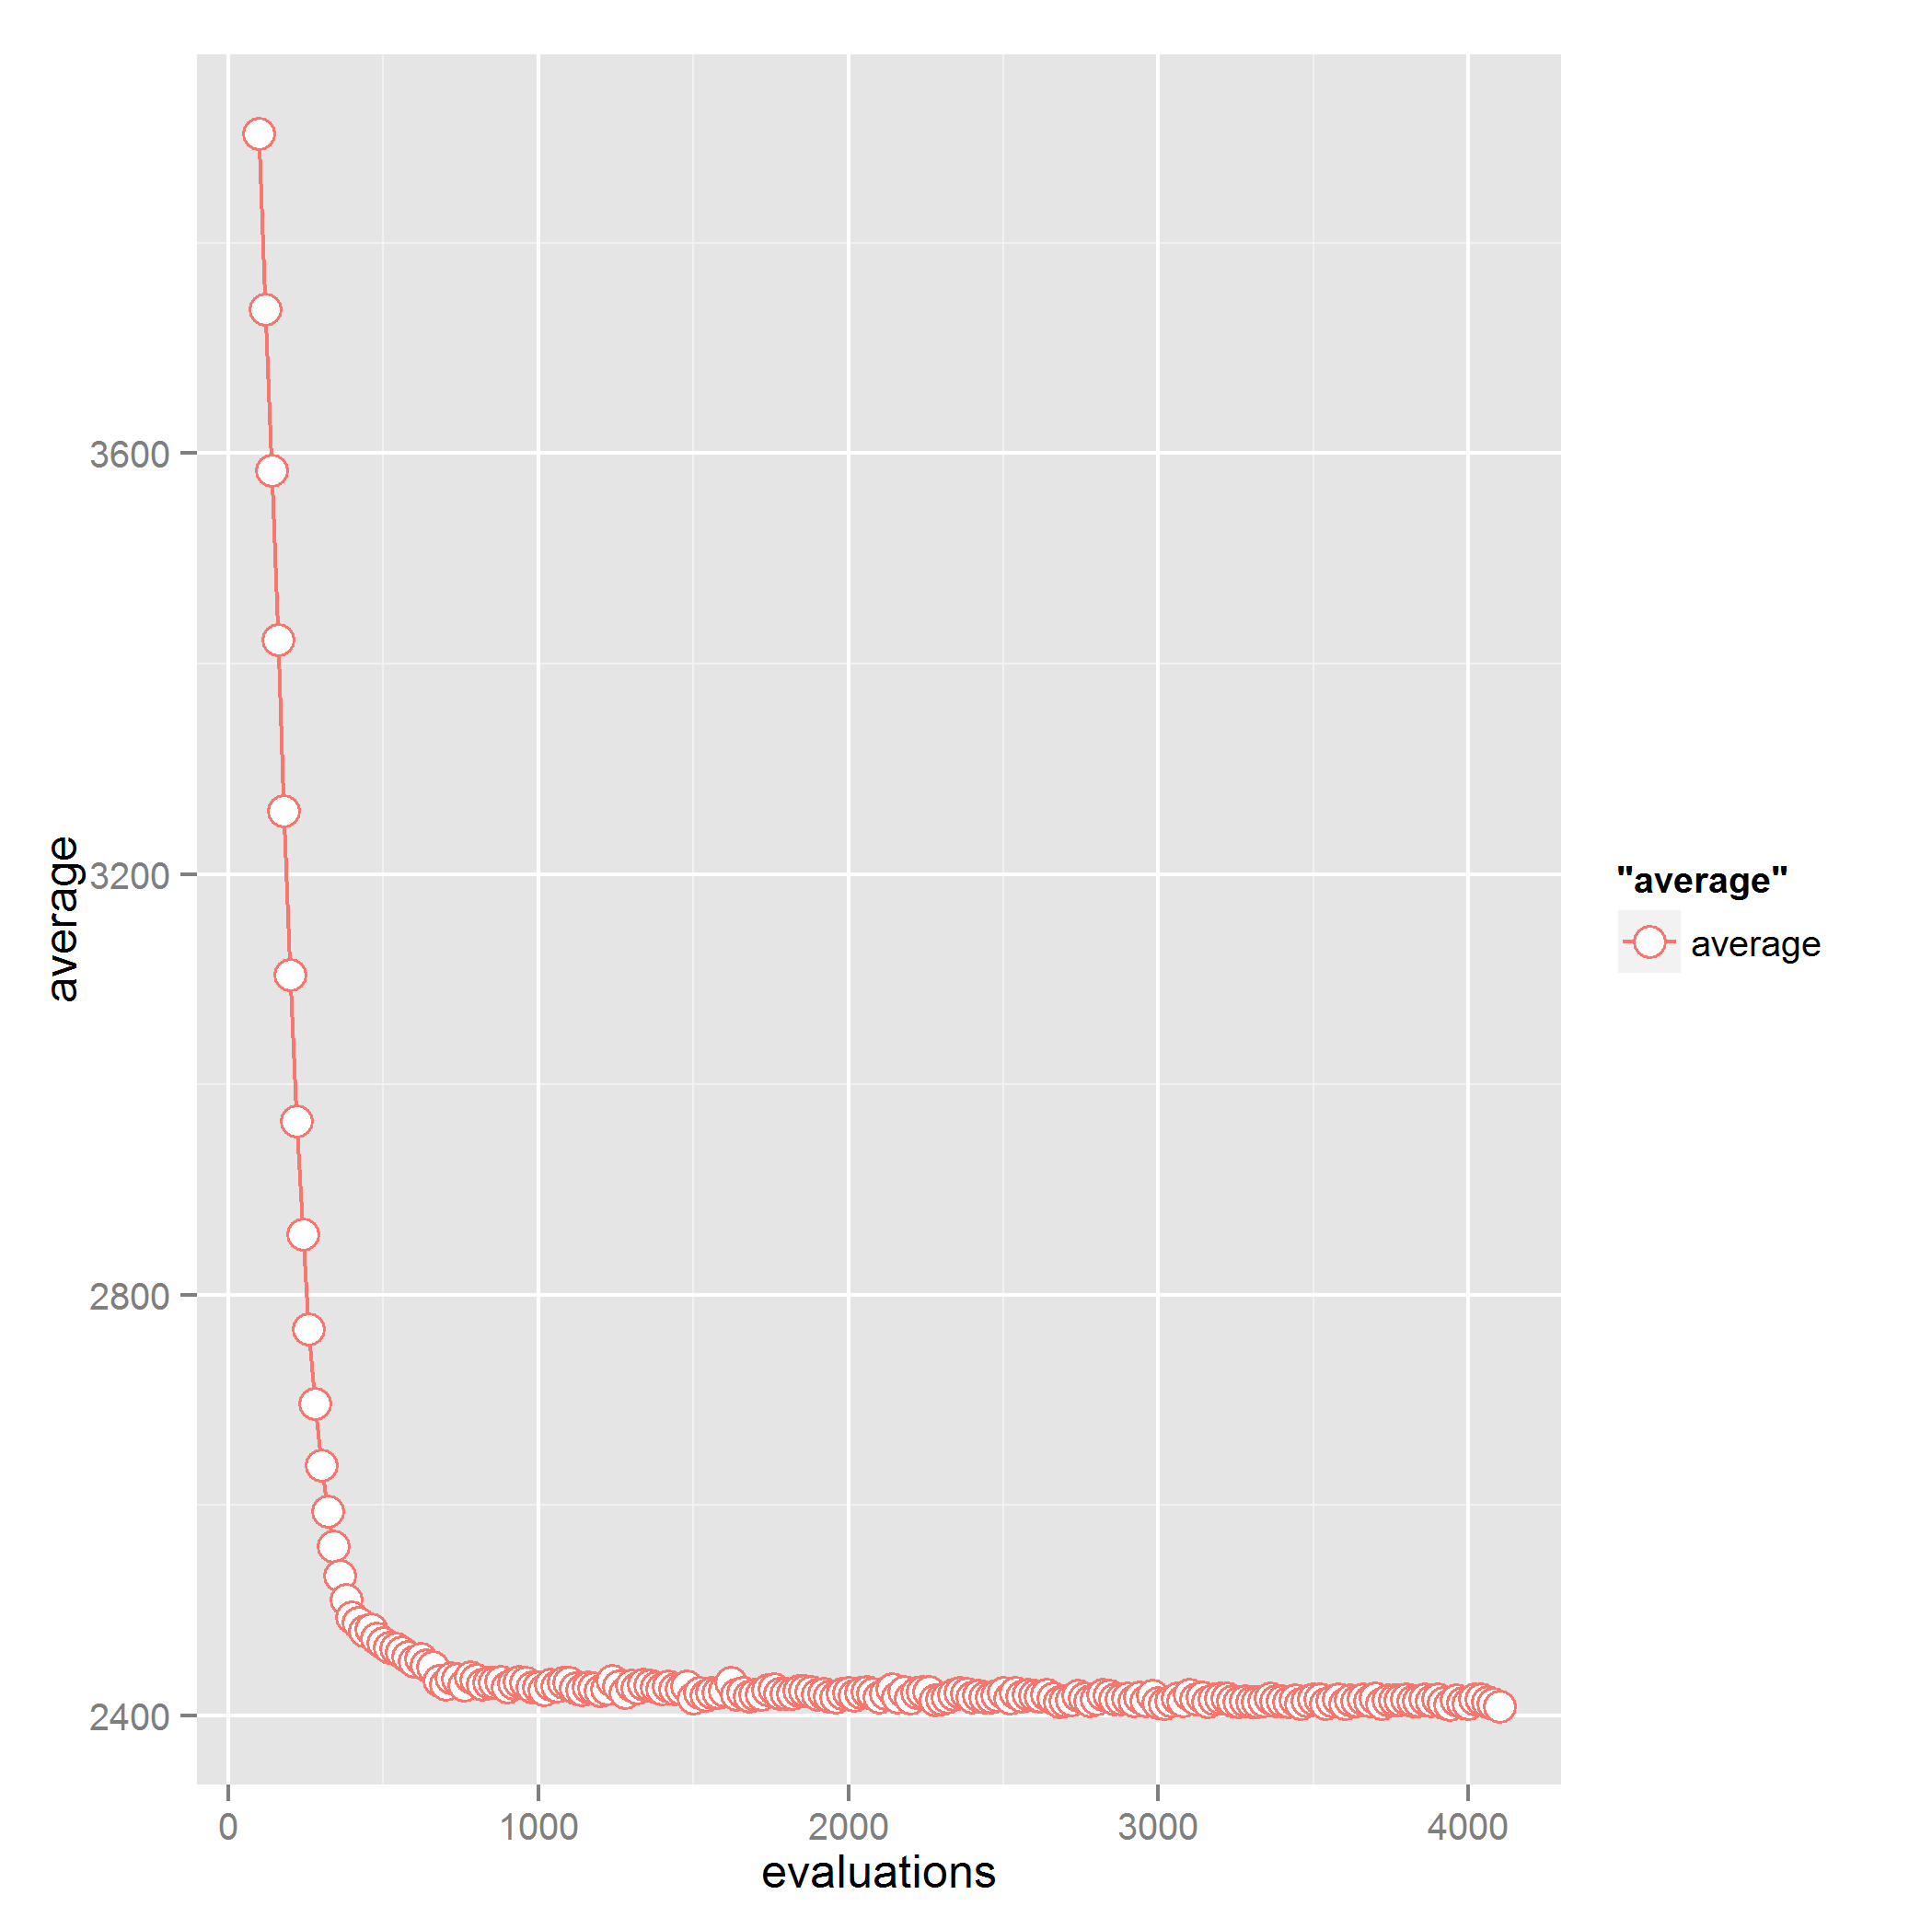
\includegraphics[]{mutation_cooling_graph0.png}

Średni rozmiar danych:

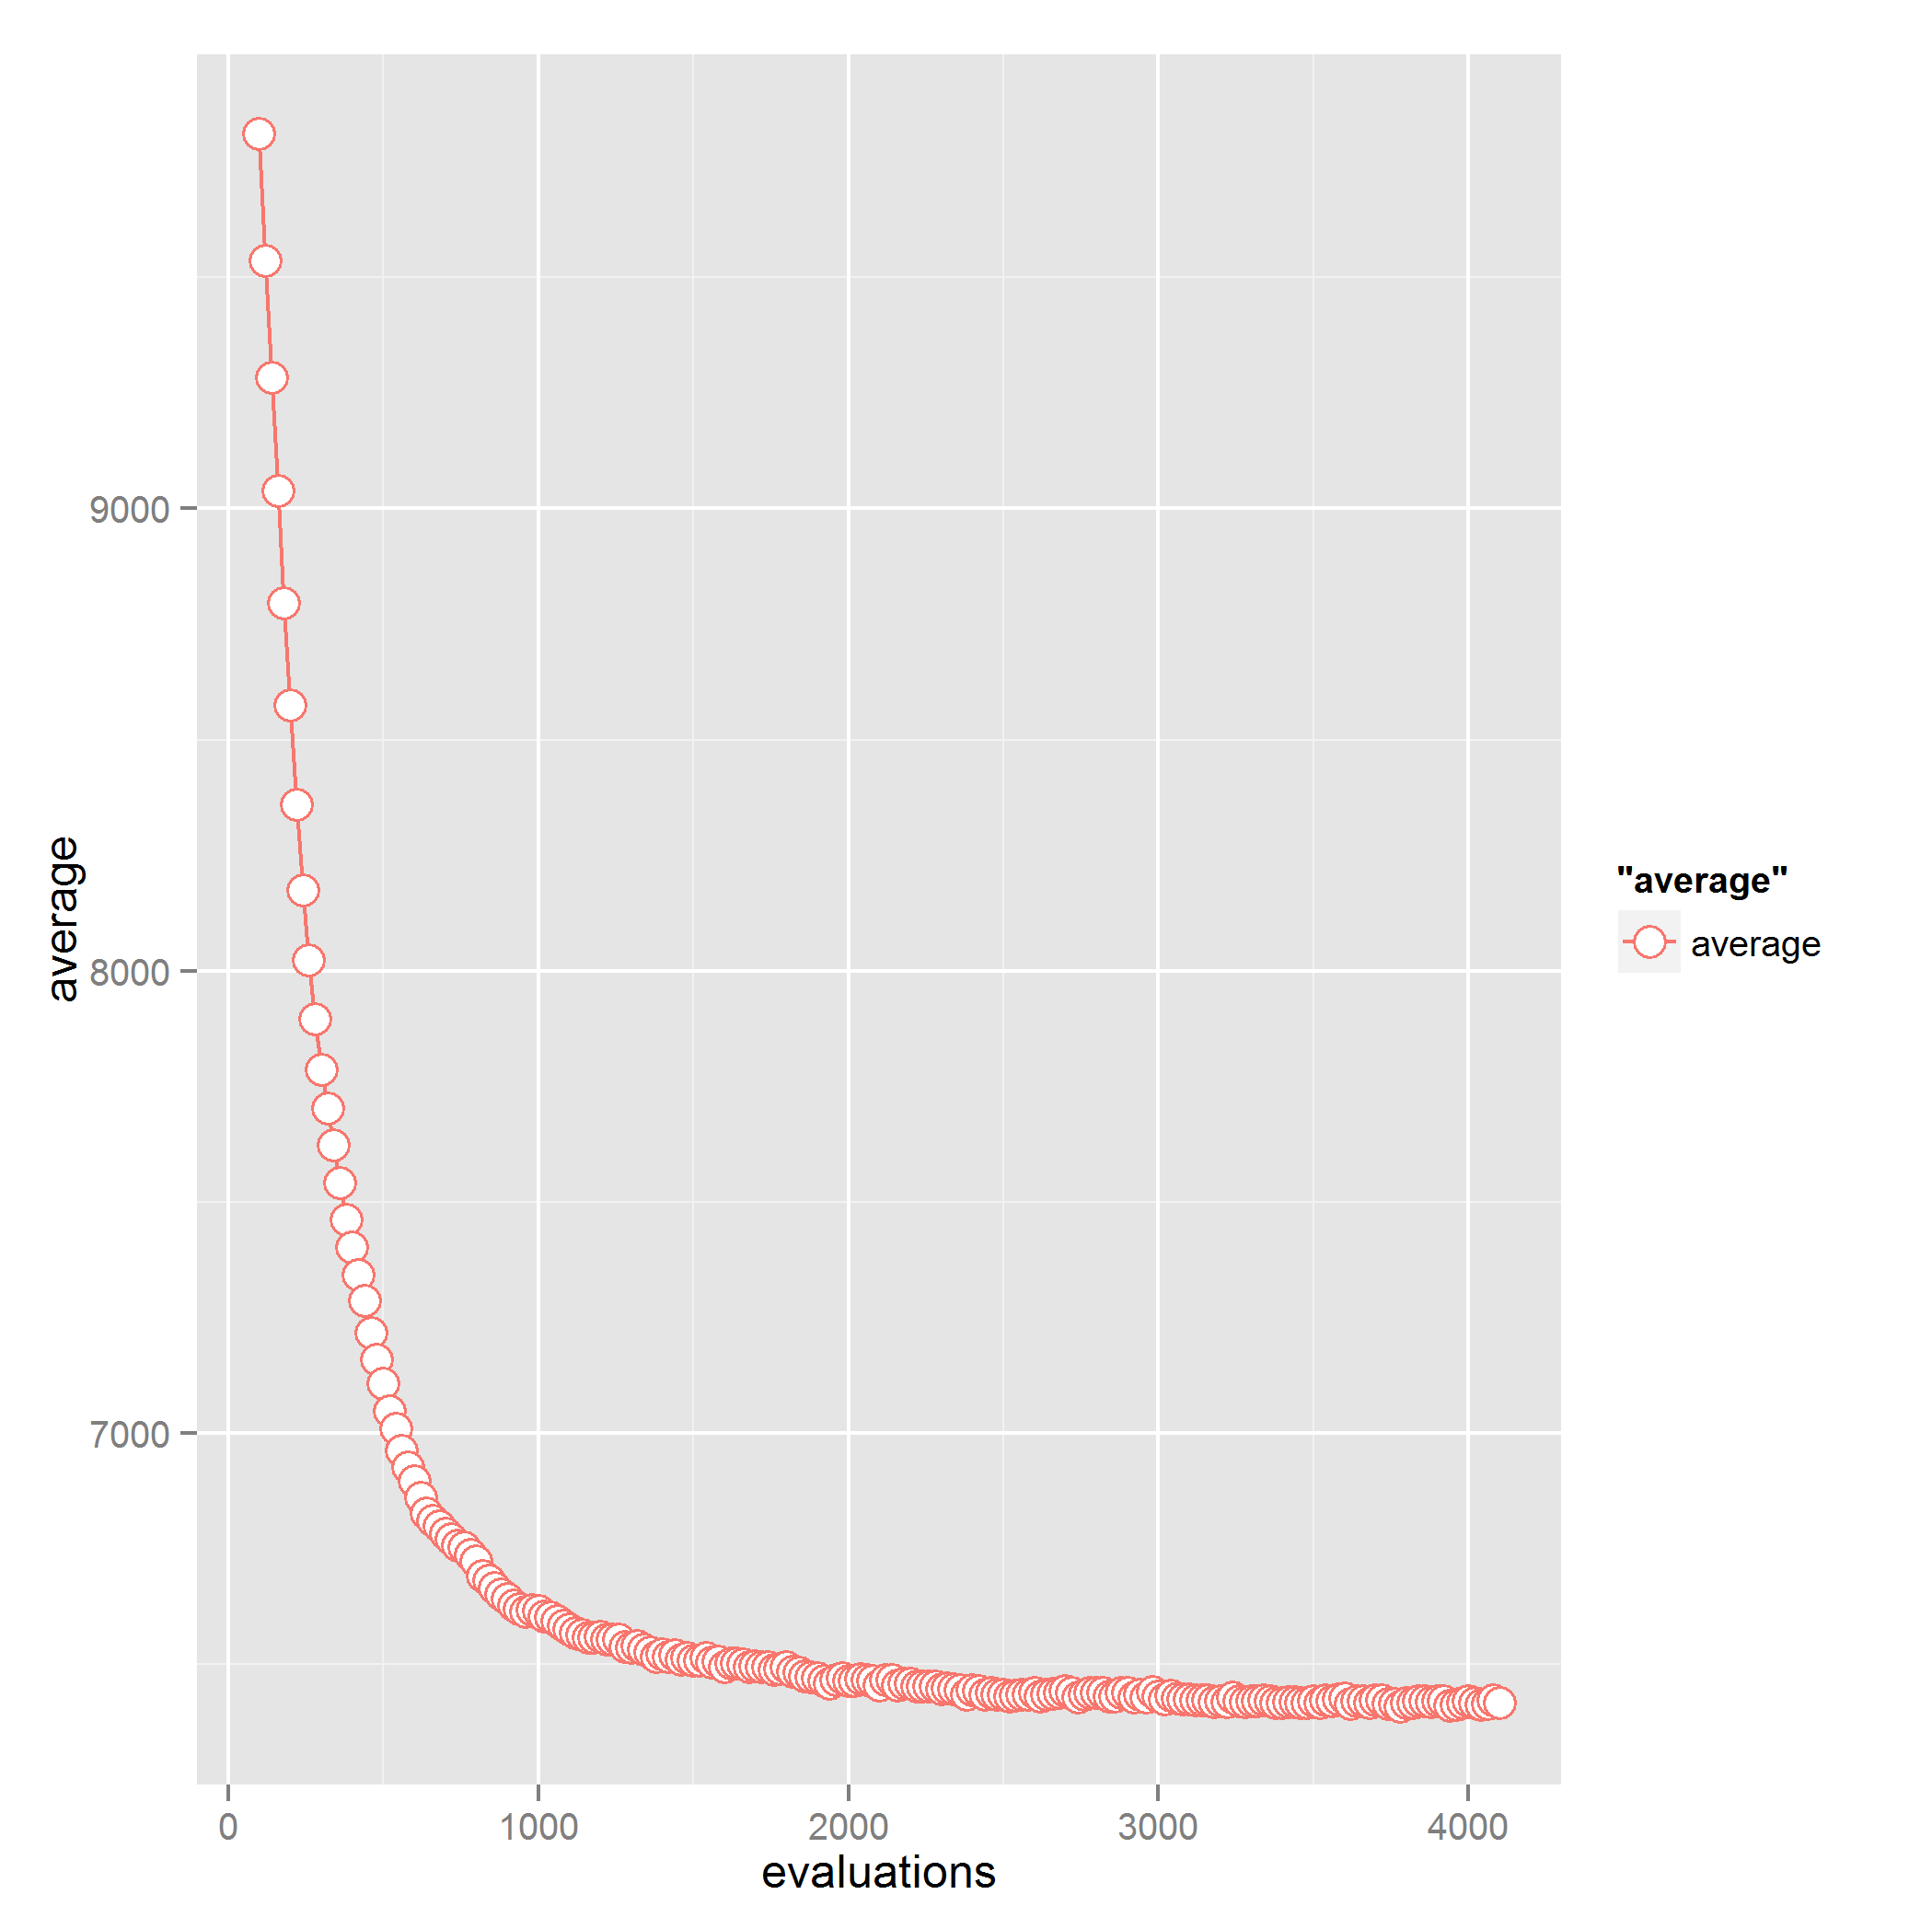
\includegraphics[]{mutation_cooling_graph1.png}

Duży rozmiar danych:

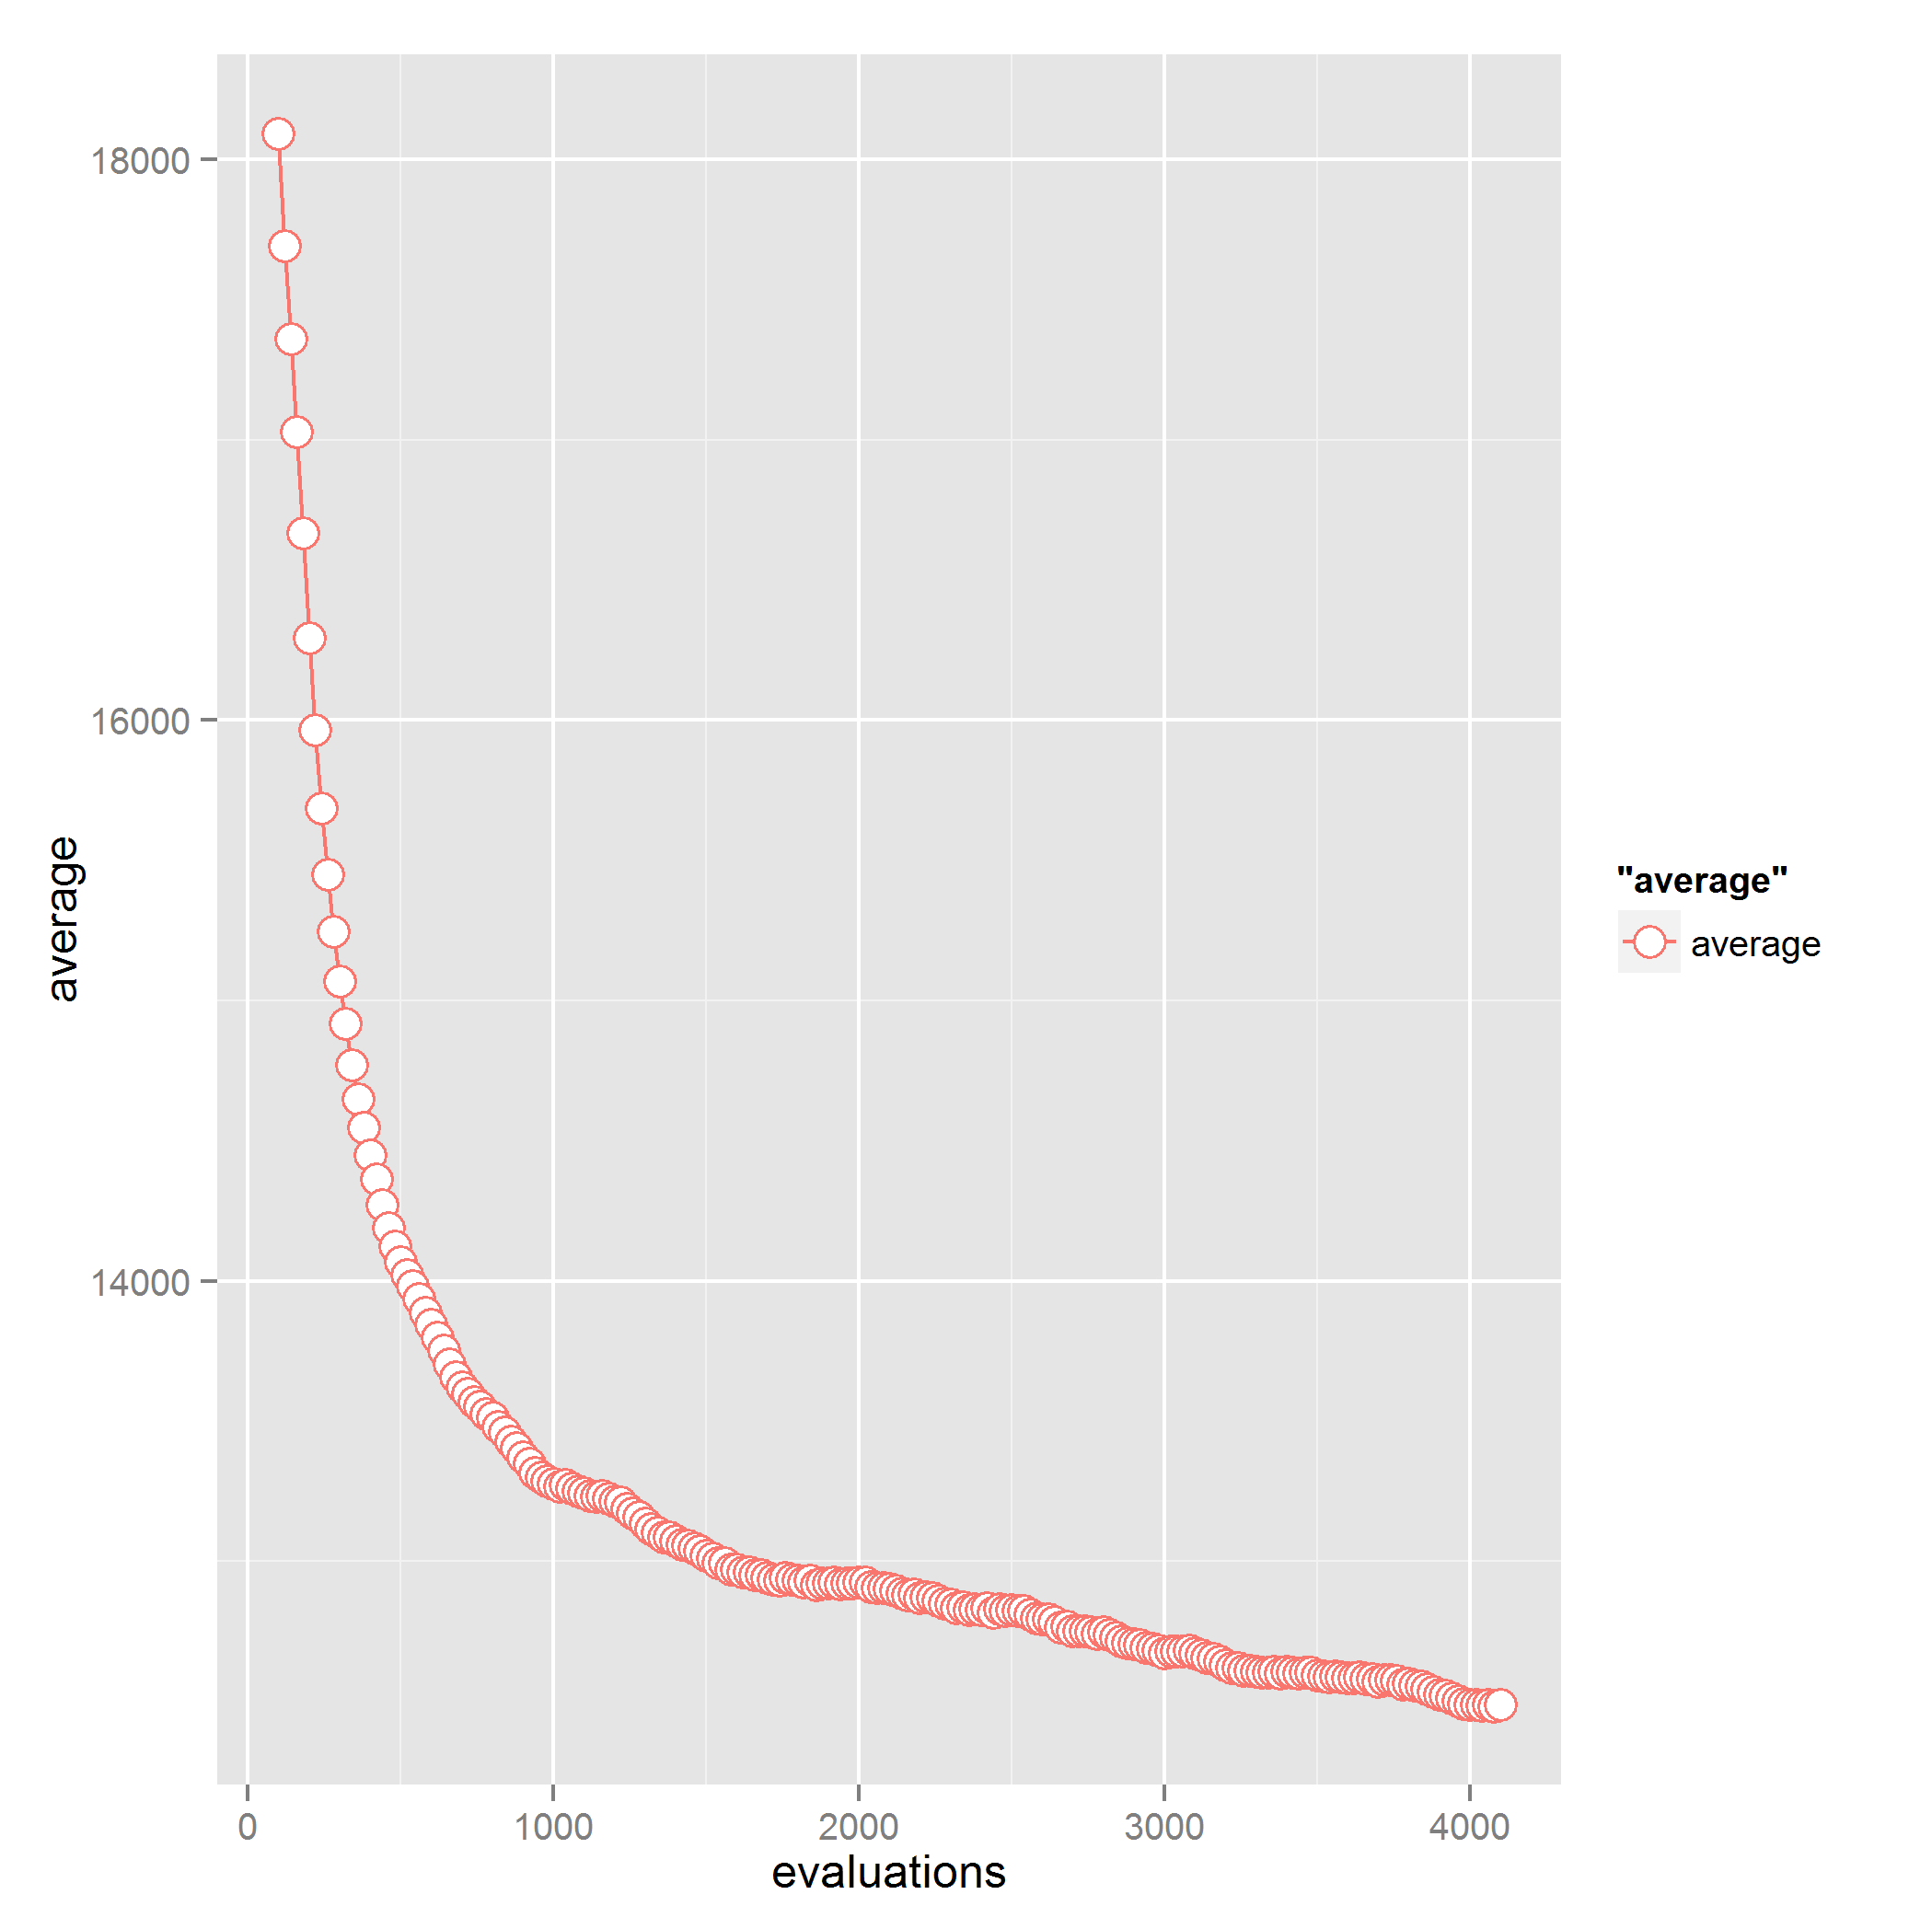
\includegraphics[]{mutation_cooling_graph2.png}

Ostatni przypadek pochodzi od hybrydy w której jako presję selekcyjną wykorzystaliśmy rozmiar turnieju. Ponieważ im większy turniej tym mniejsze prawdopodobieństwo przetrwania słabych osobników, na początku ustalilismy mały rozmiar turnieju, który stopniowo rośnie.

Mały rozmiar danych:

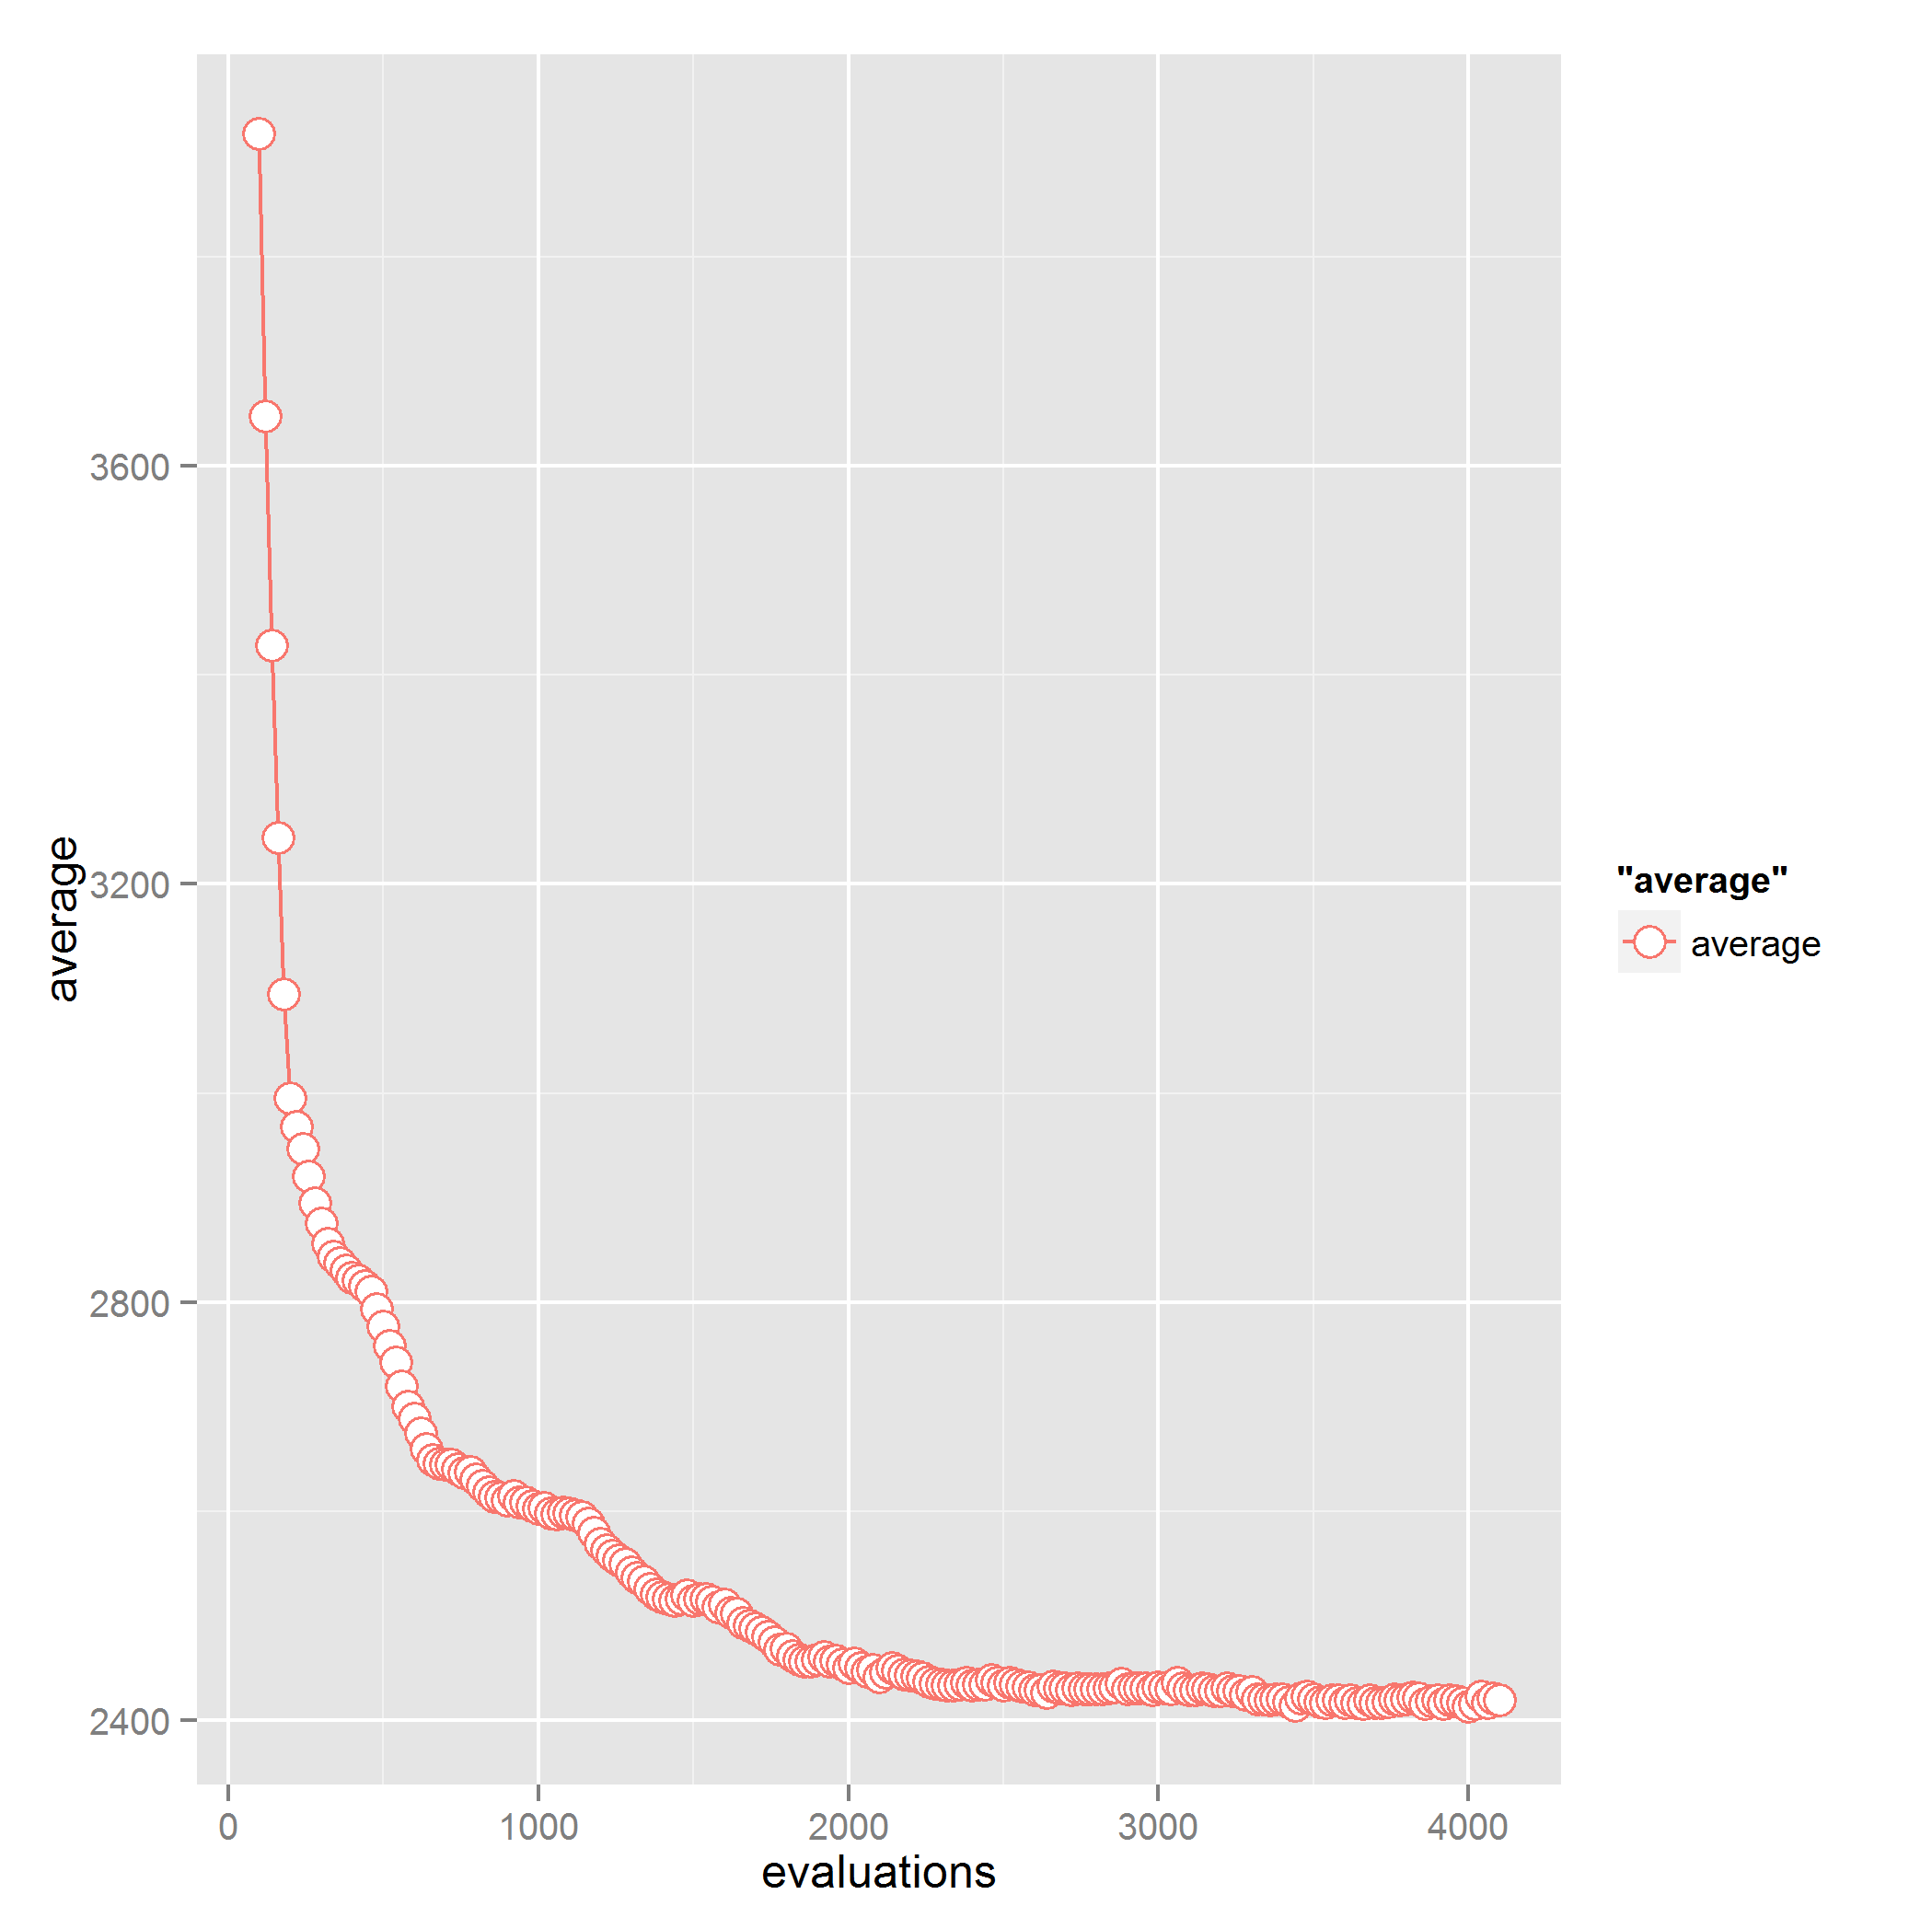
\includegraphics[]{tournament_cooling_graph0.png}

Średni rozmiar danych:

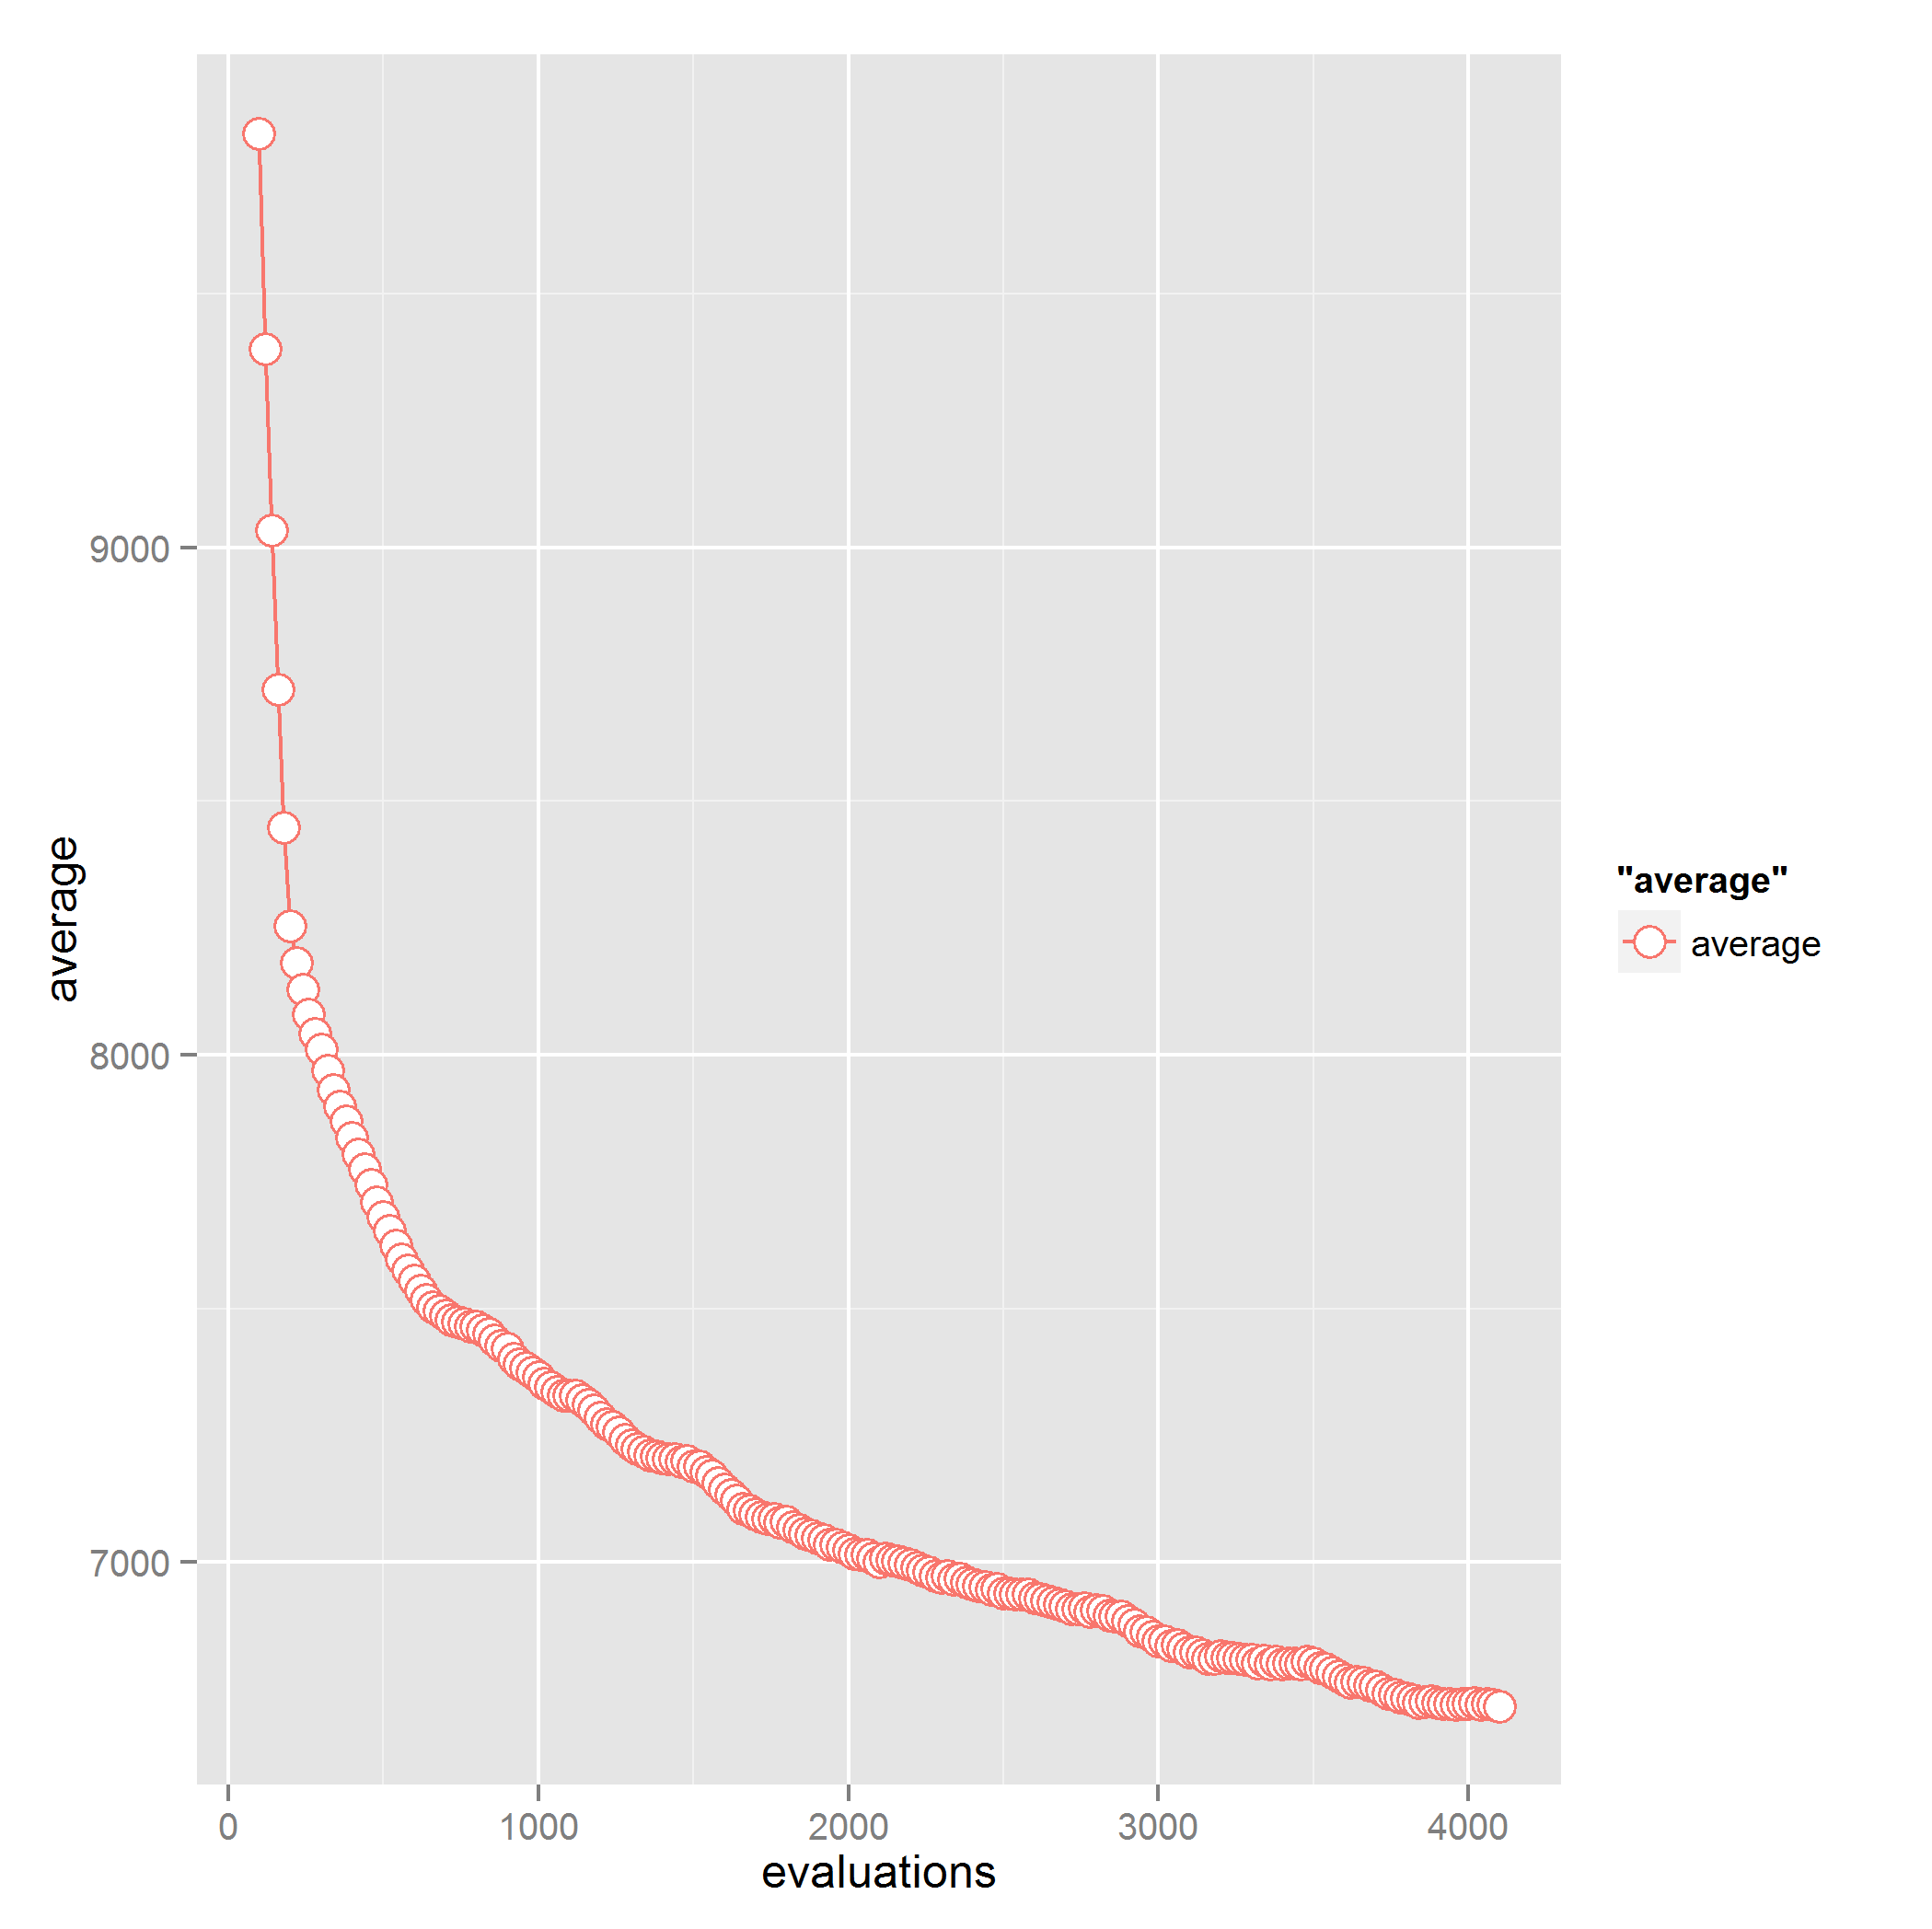
\includegraphics[]{tournament_cooling_graph1.png}

Duży rozmiar danych:

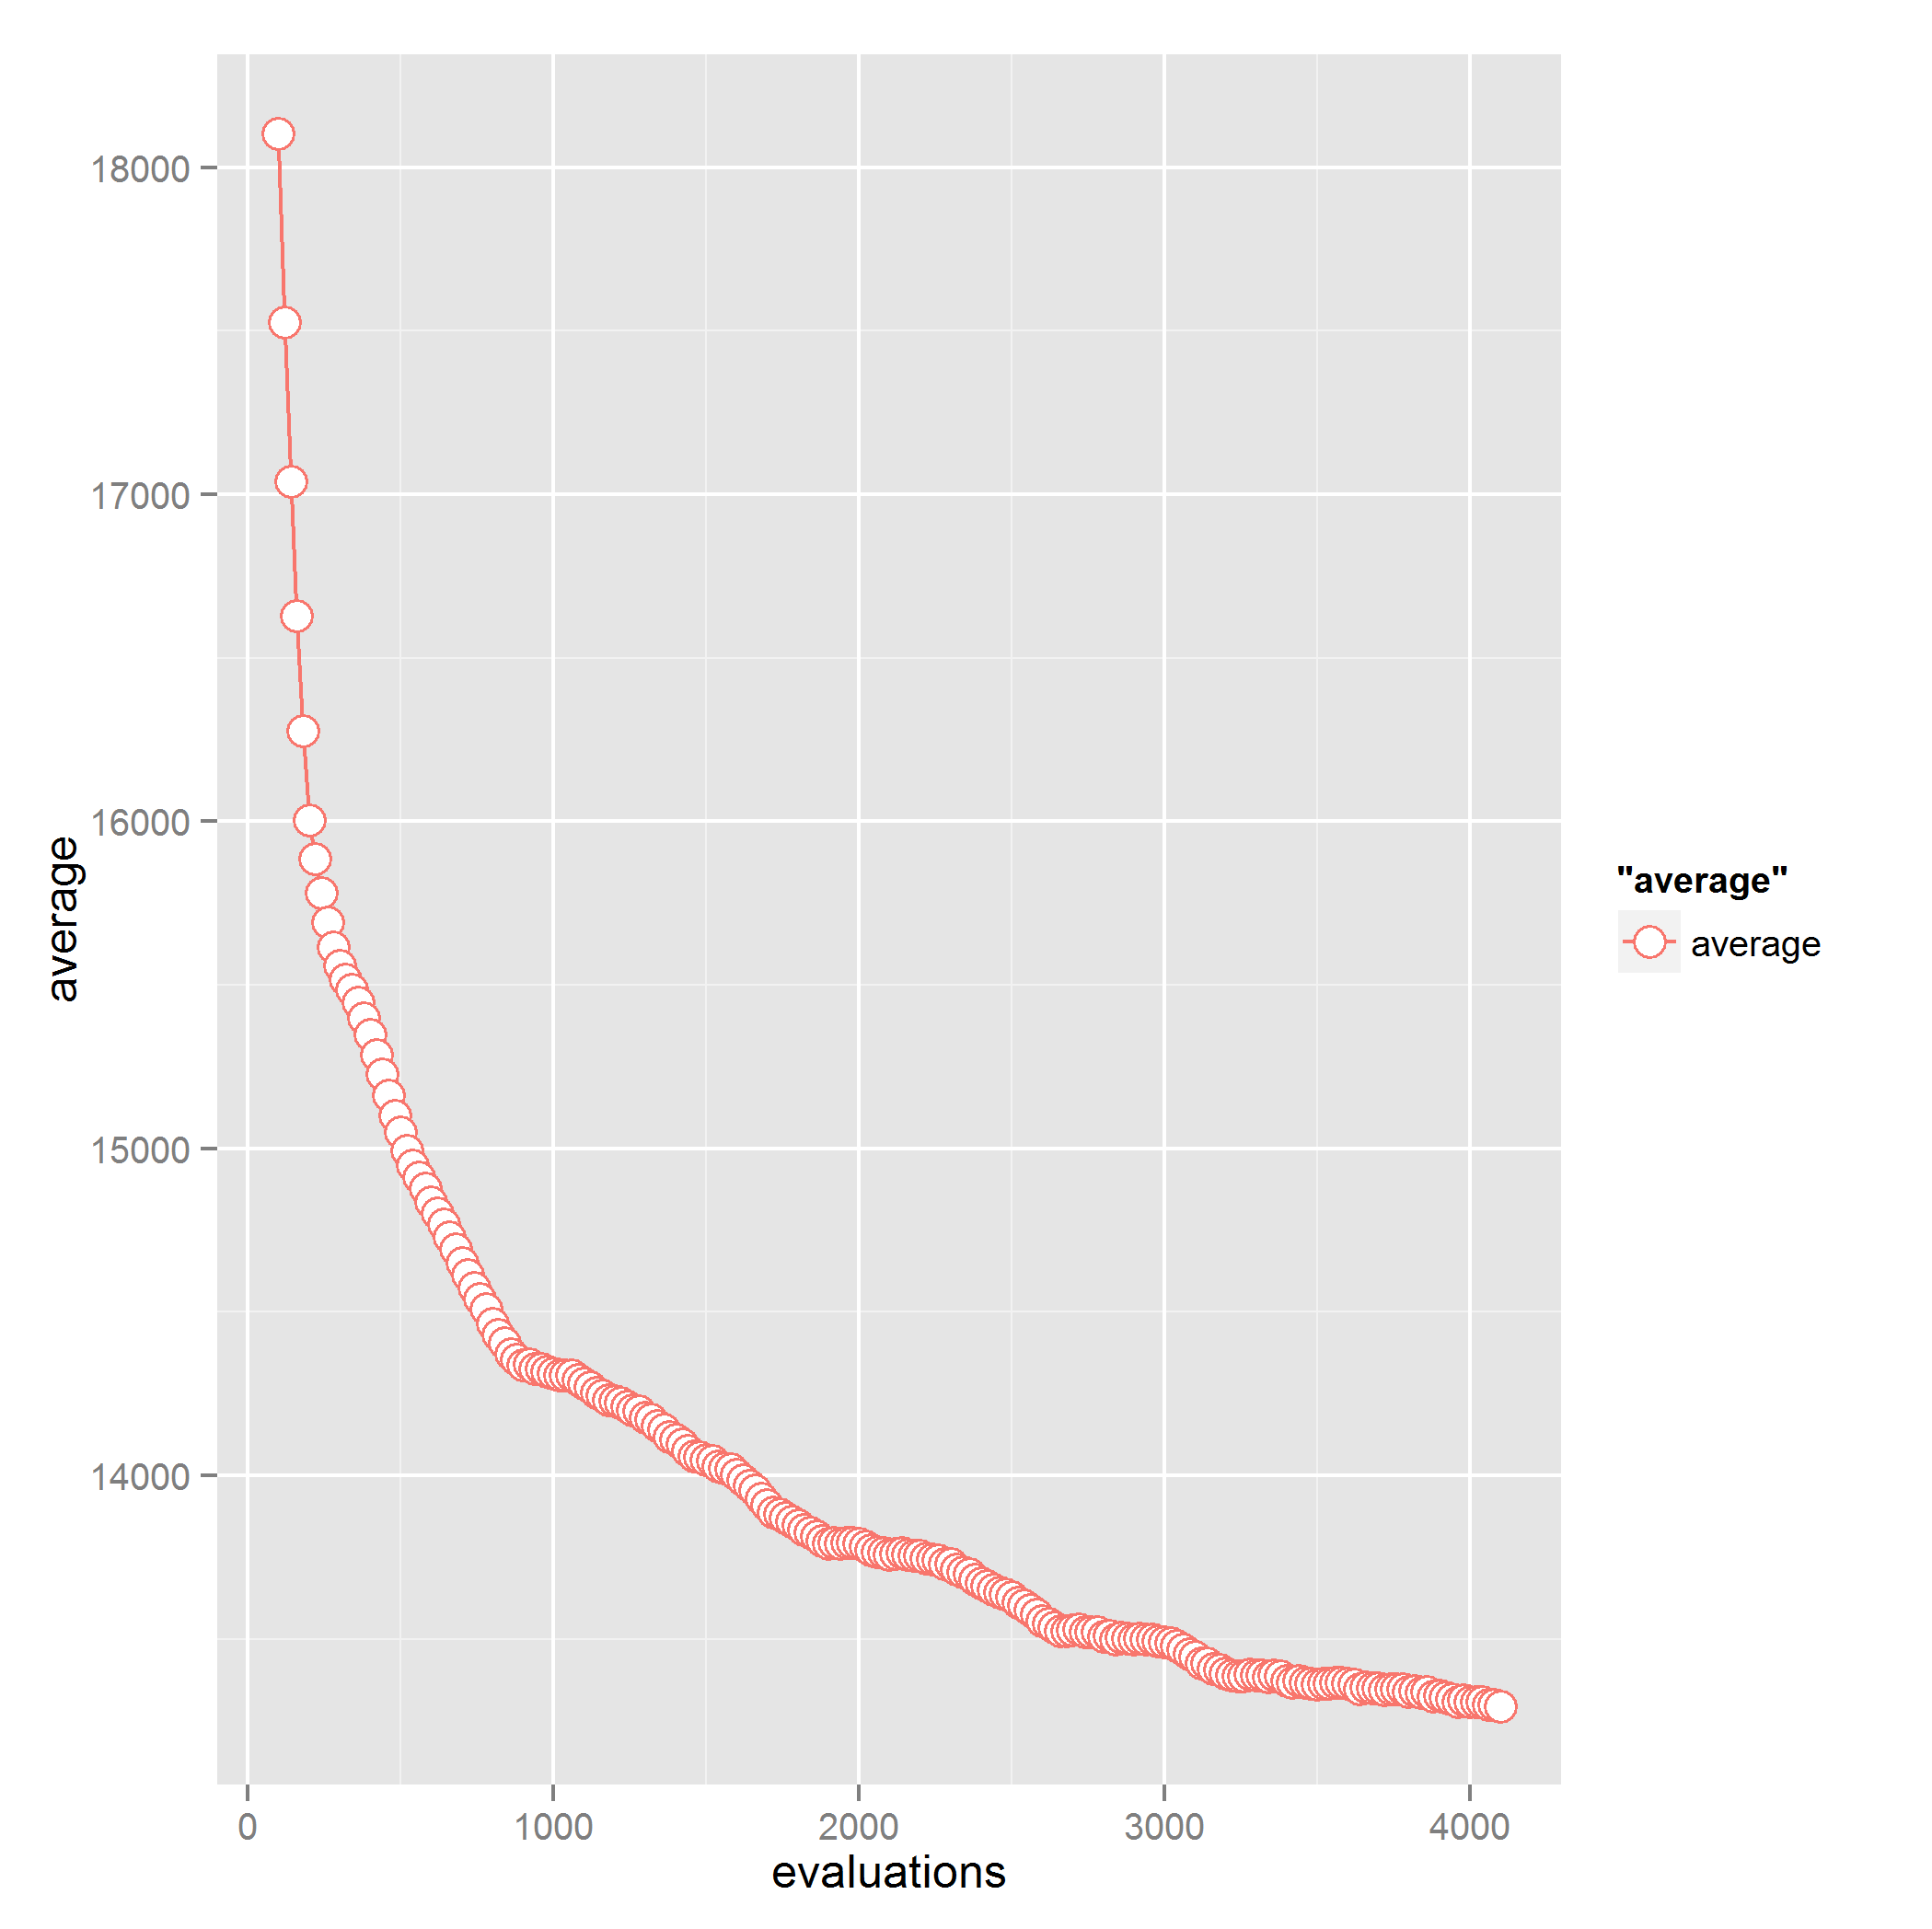
\includegraphics[]{tournament_cooling_graph2.png}

\section*{Wnioski}

Okazuje się że wbrew oczekiwaniom, najzwyklejszy algorytm genetyczny daje lepsze wyniki i jest szybciej zbieżny do optymalnego rozwiązania niż hybrydy. Obie hybrydy algorytmu genetycznego z symulowanym wyzarzaniem dają wyniki w bardzo zbliżonym czasie i są zbieżne z podobną prędkoscią. Nie jesteśmy w stanie określić jaka jest przyczyna takiego stanu rzeczy.



\bibliography{scibib}

\bibliographystyle{Science}



% Following is a new environment, {scilastnote}, that's defined in the
% preamble and that allows authors to add a reference at the end of the
% list that's not signaled in the text; such references are used in
% *Science* for acknowledgments of funding, help, etc.

% For your review copy (i.e., the file you initially send in for
% evaluation), you can use the {figure} environment and the
% \includegraphics command to stream your figures into the text, placing
% all figures at the end.  For the final, revised manuscript for
% acceptance and production, however, PostScript or other graphics
% should not be streamed into your compliled file.  Instead, set
% captions as simple paragraphs (with a \noindent tag), setting them
% off from the rest of the text with a \clearpage as shown  below, and
% submit figures as separate files according to the Art Department's
% instructions.


\clearpage

\end{document}




















